\section{~Numerical approaches} \label{chapt:num}
\newcounters

The Wave Action Equation in Cartesian (\ref{eq:bal_plane}) or spherical (\ref{eq:bal_sphere}) coordinates is the basic
equations of the wave model. However, modified versions of these equations are
used in the model, where (a) they are solved on a variable wavenumber grid
(see below), where (b) a modified versions of these equations are used to
properly described dispersion for discretized equations in selected numerical
schemes (see \para\ref{sub:xy_prop}), and where (c) sub-grid obstacles such as
islands are considered (see \para\ref{sub:xy_prop}).


\vssub
\subsection{~Spectral discretization} \label{sec:basic_num}
\vsssub


If (\ref{eq:bal_plane}) or (\ref{eq:bal_sphere}) is solved directly, an
effective reduction of spectral resolution occurs in shallow water
\citep[see][]{tol:GAOS98b}. This loss of resolution can be avoided if the
equation is solved on a variable wavenumber grid, which implicitly
incorporates the kinematic wavenumber changes due to shoaling. Such a
wavenumber grid corresponds to a spatially and temporally invariant
grid in relartive frequency \citep{tol:GAOS98b}. The corresponding local wavenumber grid can be
calculated directly from the invariant frequency grid and the dispersion
relation (\ref{eq:disp}), and hence becomes a function of the local depth
$d$. To accommodate economical calculations of $S_{nl}$ and allow a good separation of swell frequencies, a frequency discretization with 
exponentially increasing lags is adopted, so that the varying frequency resolution is proportional to the local frequency, 

%----------------------------%
% Exponential frequency grid %
%----------------------------%
% eq:sigma_grid

\begin{equation}
\sigma_{m+1} = X_\sigma \, \sigma_m \: , \label{eq:sigma_grid}
\end{equation}

\noindent
where $m$ is a discrete grid counter in $k$-space. $X_\sigma$ is defined by
the user in the input files of the program. Traditionally, in most
applications of third-generation models $X_\sigma \simeq 1.1$ is used.

The effects of a spatially varying grid will be discussed for the Cartesian
equation (\ref{eq:bal_plane}) only. Adaptation to the spherical grid is
trivial. Denoting the variable wavenumber grid with $\kappa$, the balance
equation becomes

%------------------------------%
% general equations kappa-grid %
%------------------------------%
% eq:bal_f_grid
% eq:sigma_dot

\begin{equation}
\frac{\p}{\p t} \frac{N}{c_g} +  
\frac{\p}{\p x} \frac{\dot{x} N}{c_g} + 
\frac{\p}{\p y} \frac{\dot{y} N}{c_g} + 
\frac{\p}{\p \kappa} \frac{\dot{\kappa} N}{c_g} + 
\frac{\p}{\p \theta} \frac{\dot{\theta} N}{c_g}  =
\frac{S}{\sigma c_g} \: , \label{eq:bal_f_grid} \end{equation} \begin{equation}
\dot{\kappa} \:\frac{\p k}{\p \kappa} =
     c_g^{-1} \frac{\p \sigma}{\p d} \left (
    \frac{\p d}{\p t} + {\bf U} \cdot \nabla_x d \: \right ) -
    {\bf k} \cdot \frac{\p {\bf U}}{\p s}
\: . \label{eq:sigma_dot}
\end{equation}

\noindent

\vssub
\subsection{~Splitting of the wave action equation} \label{sec:basic_num}
\vsssub

In \ww, equation (\ref{eq:bal_f_grid}) is solved using a fractional step method. 
The first step treats the temporal variations of
the depth, and corresponding changes in the wavenumber grid. As is discussed
by \cite{tol:GAOS98b}, this step can be invoked sparsely. By splitting off
effects of (temporal) water level variations, the grid becomes invariant, and
the depth becomes quasi-steady for the remaining fractional steps. Other
fractional steps consider spatial propagation, intra-spectral propagation and
source terms. Starting with version 5.10, the source term $S$ is further split into 
non-ice $S_{no~ice}$ and ice $S_{ice}$ source term. For a single model grid, the following sequence of integration  is performed 
by the {\code W3WAVE} routine,
\begin{itemize}
 \item[1.] update of water level 
 \item[2.] intra-spectral part 1: integration over $\Delta t_g/2$ of  $\frac{\p}{\p t} \frac{N}{c_g} + \frac{\p}{\p \kappa} \frac{\dot{\kappa} N}{c_g} + \frac{\p}{\p \theta} \frac{\dot{\theta} N}{c_g}  =0 $ 
 \item[3.] spatial propagation : integration over $\Delta t_g$ of $\frac{\p}{\p t} \frac{N}{c_g} +  
\frac{\p}{\p x} \frac{\dot{x} N}{c_g} + 
\frac{\p}{\p y} \frac{\dot{y} N}{c_g}  = 0$
 \item[4.] intra-spectral part 2: integration over $\Delta t_g/2$ of  $\frac{\p}{\p t} \frac{N}{c_g} + \frac{\p}{\p \kappa} \frac{\dot{\kappa} N}{c_g} + \frac{\p}{\p \theta} \frac{\dot{\theta} N}{c_g}  =0 $ 
 \item[5.] source term integration : integration over $\Delta t_g$ of $\frac{\p}{\p t} \frac{N}{c_g}   = \frac{S_{no~ice}}{\sigma c_g}$
 \item[6.] ice source term integration : integration over $\Delta t_g$ of $\frac{\p}{\p t} \frac{N}{c_g}   = \frac{S_{ice}}{\sigma c_g}$ 
\end{itemize}
The succession of these 6 steps is, in the limit $\Delta t_g \rightarrow 0$, equivalent to the integration of eq. (\ref{eq:bal_f_grid}) over a global 
time step $\Delta t_g$. 

This splitting in multiple steps allows an  efficient 
vectorization and parallelization at the same time. The time splitting furthermore
allows for the use of separate partial or dynamically adjusted time steps in
the different fractional steps of the model. \ws\ makes a distinction between
4 different time steps. \label{dt_list}

\begin{list}{xx}{\itemsep 0mm \parsep 0mm \rightmargin 5mm}

\item[1)] The `global' time step $\Delta t_g$, is the common step of all the splitted sub-integrations. In that sense, 
it is the smallest time step for which a physically meaningful solution can be obtained, because all terms in the equation have been 
integrated. As a result, this is a possible time step for evaluating model output or coupling with other models, 
and, in the case of a multi-grid system,  it is the time step at which communication 
between grids is performed. In the case of a forced -- not coupled -- model, input winds and currents are
interpolated at this global step. This time step is provided by the user in the input file of {\code ww3\_grid}, but can be reduced
within the model to reach a requested input or output time.

\item[2)] The second time step is the time step for spatial propagation. This is not used for triangular-based 
grids, for which the advection step is -- in the case of explicit schemes -- adjusted internally for each spectral component. For other grid types, the
user supplies a reference maximum propagation time step for the lowest model
frequency $\Delta t_{p,r}$, assuming no currents, and no grid motion. For the
frequency with counter $m$, the maximum time step $\Delta t_{p,m}$ is
calculated within the model as

%-------------------------%
% Time stepping equations %
%-------------------------%
% eq:dtpl

\begin{equation}
\Delta t_{p,m} = \frac{{\dot{x}}_{p,r}}{{\dot{x}}_{p,m}} \Delta t_{p,r}
\: . \label{eq:dtpl} \end{equation}

\noindent
where $\dot{x}_{p,r}$ is the maximum advection speed for the longest waves
without currents or grid motion, and $\dot{x}_{p,m}$ is the actual maximum
advection speed (including current) for frequency $m$. If the propagation time
step is smaller than the global time step, the propagation effects are
calculated with a number of successive smaller time steps. This generally
implies that several partial time steps are used for the lowest frequency, but
that the highest frequencies are propagated over the interval $\Delta t_g$
with a single calculation. The latter results in a significantly more
efficient model, particularly if higher-order accurate propagation schemes are
used. Note that $\Delta t_{p,m}$ may be defined bigger than $\Delta t_g$, and
that this has potential impact in model economy for cases with (strong)
currents.

\item[3)] The third time step is the time step for intra-spectral
propagation. For large-scale and deep-water grids this time step can generally
be taken equal to the global time step $\Delta t_g$. For shallow water grids,
smaller intra-spectral propagation time steps allow for larger effects of
refraction within the stability constraints of the scheme. Note that the order
of invoking spatial and intra-spectral propagation is alternated to enhance
numerical accuracy. If strong refraction of long period swells occur, this may
result in a notable undulation of mean wave parameters. This can be avoided by
setting this time step to an even integer fraction of $\Delta t_g$.

\item[4)] The final time step is the time step for the integration of the
source terms, which is dynamically adjusted for each separate grid point and
global time step $\Delta t_g$ (see \para~\ref{sub:source}). This results in
more accurate calculations for rapidly changing wind and wave conditions, and
a more economical integration for slowly varying conditions. In order to limit the 
calculation time, a minimum time step is defined by the user. 

\end{list}

\vspace{\baselineskip} \noindent 

The following sections deal with the separate steps in the fractional step
method, and various subjects associated with this.  The main issue are covered
in \para\ref{sub:num_depth}, which addresses treatment of temporal variations
of the water depth, \para\ref{sub:xy_prop}, which addresses spatial
propagation, \para\ref{sub:spec}, which addresses intra-spectral propagation,
and \para\ref{sub:source} addresses the numerical integration of the source
terms.  Sections \ref{sub:num_w_c} and following deal with additional
numerical approaches and techniques, covering the treatment of winds and
currents, including tides (\ref{sub:num_w_c}, \ref{sub:num_tide}), treatment
of ice (\ref{sub:num_ice}), spectral partitioning and the corresponding
tracking of wave systems in space and time (\ref{sub:num_part},
\ref{sub:num_track}), and nesting (\ref{sub:num_nest}).

\vssub
\subsection{~Depth variations in time} \label{sub:num_depth}
\vssub

Temporal depth variations result in a change of the local wavenumber
grid. Because the wavenumber spectrum is invariant with respect to temporal
changes of the depth, this corresponds to a simple interpolation of the
spectrum from the old grid to the new grid, without changes in the spectral
shape. As discussed above, the new grid simply follows from the globally
invariant frequency grid, the new water depth $d$ and the dispersion relation
Eq. (\ref{eq:disp}). The time step of updating the water level is generally
dictated by physical time scales of water level variations, but not by
numerical considerations \citep{tol:GAOS98b}.

The interpolation to the new wavenumber grid is performed with a simple
conservative interpolation method. In this interpolation the old spectrum is
first converted to discrete action densities by multiplication with the
spectral bin widths. This discrete action then is redistributed over the new
grid cf.\ a regular linear interpolation. The new discrete actions then are
converted into a spectrum by division by the (new) spectral bin widths. The
conversion requires a parametric extension of the original spectrum at high
and low frequencies because the old grid generally will not completely cover
the new grid. Energy/action in the old spectrum at low wavenumbers that are
not resolved by the new grid is simply removed. At low wavenumbers in the new
grid that are not resolved by the old grid zero energy/action is assumed. At
high wavenumbers in the new grid the usual parametric tail is applied if
necessary. The latter correction is rare, as the highest wavenumbers usually
correspond to deep water.

In practical applications the grid modification is usually relevant for a
small fraction of the grid points only. To avoid unnecessary calculations, the
grid is transformed only if the smallest relative depth $kd$ in the discrete
spectrum is smaller than 4. Furthermore, the spectrum is interpolated only if
the spatial grid point is not covered by ice, and if the largest change of
wavenumber is at least $0.05 \Delta k$.

\vssub
\subsection{~Spatial propagation} \label{sub:xy_prop}
\vssub
\subsubsection{~General concepts}
\vsssub

Spatial propagation in \ws\ is described by the first terms of
Eq. (\ref{eq:bal_f_grid}). For spherical coordinates
[Eq. (\ref{eq:bal_sphere})], the corresponding spatial propagation step
becomes

%----------------------------%
% Step : Spatial propagation %
%----------------------------%
% eq:step_xy_prop

\begin{equation}
\frac{\p \cN}{\p t} + \frac{\p}{\p \phi} \, \dot{\phi} \cN +
\frac{\p}{\p \lambda} \, \dot{\lambda} \cN = 0
\: , \label{eq:step_xy_prop} 
\end{equation}

\noindent 
where the propagated quantity $\cN$ is defined as $\cN \equiv N \, c_g^{-1} \,
\cos\phi$. For the Cartesian grid, a similar equation is found propagating
$\cN \equiv N \, c_g^{-1}$. In this section equations for the more complicated
spherical grid are presented only. Conversion to a Cartesian grid is generally
a simplification and is trivial.

Equation~(\ref{eq:step_xy_prop}) in form is identical to the conventional
deep-water propagation equation, but includes effects of both limited depths
and currents. At the land-sea boundaries, wave action propagating toward the
land is assumed to be absorbed without reflection, and waves propagating away
from the coast are assumed to have no energy at the coastline. For so-called
`active boundary points' where boundary conditions are prescribed, a similar
approach is used. Action traveling toward such points is absorbed, whereas
action at the boundary points is used to estimate action fluxes for components
traveling into the model.

The spatial grids can use two different coordinate systems, either a 'flat'
Cartesian coordinate system typically used for small scale and idealized test
applications, and a spherical (latitude-longitude) system used for most
real-world applications. In model version 3.14, the coordinate system was
selected at compile time with the {\code XYG} or {\code LLG} switches. In more
recent model versions, the grid type is now a variable defined in {\file
ww3\_grid} and stored in the {\file mod\_def.ww3} file.

Up to model version 3.14, \ws\ considered only regular discrete grids,
where the two main grid axes ($x,y$) are discretized using constant
increments $\Delta x$ and $\Delta y$. In model version \WWver\
additional options have been included, including curvilinear grids and
unstructured grids. In the following sections these grid approached
will be discussed, before additional propagation issues are addressed,
covering the Garden Sprinkler Effect (\ref{sub:num_GSE}), continuously
moving grids (\ref{sub:num_move}) unresolved islands
(\ref{sub:num_obst}), and rotated grids (\ref{sub:num_space_rotagrid})

\vssub
\subsubsection{~Traditional regular grids} \label{sub:num_space_trad}

\noindent
Propagation schemes for traditional regular grids are selected at compile time
using switches.  Several schemes are available in \ws. These schemes are
described in order of complexity below.

\pb
\addcontentsline{toc}{subsubsection}{\strut \hspace{24mm} First-order scheme}

\vspace{\baselineskip} 
\vspace{\baselineskip} 
\noindent {\bf First-order scheme}

\opthead{PR1}{\ws}{H. L. Tolman}

\noindent
A simple and cheap first order upwind scheme has been included, mainly for
testing during development of \ws. To assure numerical conservation of action,
a flux or control volume formulation is used. The flux between grid points
with counters $i$ and $i-1$ in $\phi$-space $(\cF_{i,-})$ is calculated as

% ------ First order scheme ------- %
% eq:1up_xy_1        Basic flux
% eq:1up_xy_2        Boundary velocity
% eq:1up_xy_3        Upstream value

\begin{equation}
\cF_{i,-} = \left [ \: \dot{\phi}_b \: \cN_u \: \right ]^n_{j,l,m}
\: , \label{eq:1up_xy_1} \end{equation} \begin{equation}
\dot{\phi}_b = 0.5 \: \left ( \dot{\phi}_{i-1} + \dot{\phi}_i 
\: \right )_{j,l,m} \: , \label{eq:1up_xy_2}
\end{equation} \begin{equation}
\cN_u = \left \{ \begin{array}{ccc}
\cN_{i-1} & \mbox{for} & \dot{\phi}_b \geq 0 \\
\cN_i     & \mbox{for} & \dot{\phi}_b   <  0
\end{array} \right . \: , \label{eq:1up_xy_3}
\end{equation}

\noindent
where $j$, $l$ and $m$ are discrete grid counters in $\lambda$-, $\theta$- and
$k$-spaces, respectively, and $n$ is a discrete time step
counter. $\dot{\phi}_b$ represents the propagation velocity at the `cell
boundary' between points $i$ and $i-1$, and the subscript $u$ denotes the
`upstream' grid point. At land-sea boundaries, $\dot{\phi}_b$ is replaced by
$\dot{\phi}$ at the sea point. Fluxes between points $i$ and $i+1$
$(\cF_{i,+})$ are obtained by replacing $i-1$ with $i$ and $i$ with
$i+1$. Fluxes in $\lambda$-space are calculated similarly, changing the
appropriate grid counters and increments.  The `action density' $(\cN^{n+1})$
at time $n+1$ is estimated as

% eq:1up_xy_tot

\begin{equation}
\cN_{i,j,l,m}^{n+1} = \cN_{i,j,l,m}^n
  + \frac{\Delta t}{\Delta \phi   } \left [ \cF_{i,-} - \cF_{i,+} \right ]
  + \frac{\Delta t}{\Delta \lambda} \left [ \cF_{j,-} - \cF_{j,+} \right ]
\: , \label{eq:1up_xy_tot}
\end{equation}

\noindent
where $\Delta t$ is the propagation time step, and $\Delta \phi$ and $\Delta
\lambda$ are the latitude and longitude increments, respectively. Equations
(\ref{eq:1up_xy_1}) through (\ref{eq:1up_xy_3}) with $\cN=0$ on land and
applying Eq. (\ref{eq:1up_xy_tot}) on sea points only automatically invokes
the required boundary conditions.

Note that Eq.~(\ref{eq:1up_xy_tot}) represents a two-dimensional
implementation of the scheme, for which the norm of the actual advection
vectors needs to be used in Eq.~(\ref{eq:dtpl}). Note furthermore, that this
implies a CFL criterion for the full equation, which is generally more
stringent than that for a scheme where $\lambda$ and $\phi$ propagation are
treated separately as in the third order schemes discussed below. For a grid
with equal increments in both directions, this results in a maximum time step
that is a factor $1/\sqrt{2}$ smaller for the first order scheme than for the
third order schemes.
\addcontentsline{toc}{subsubsection}{\strut \hspace{24mm} Second order scheme (UNO)}

\vspace{\baselineskip} \noindent {\bf Second order scheme (UNO)}

\opthead{UNO}{???}{J.-G. Li}

\noindent
\noindent

The upstream non-oscillatory 2nd order (UNO2) advection scheme \citep{art:Li08} is an extension of the MINMOD scheme \citep{bk:Roe85}. In the UNO2
scheme, the interpolated wave action value at the mid-flux point for
the cell face between cell \emph{i}-1 and cell \emph{i} is given by

\begin{equation}
N_{i-}^{*}=N_{c}+sign\left(N_{d}-N_{c}\right)\frac{\left(1-C\right)}{2}\min\left(|N_{u}-N_{c}|,|N_{c}-N_{d}|\right)
\label{eq:UNO2regular}
\end{equation}
where \emph{i}- is the cell face index; $C=\left|\dot{\phi_{b}}\right|\Delta t/\Delta\phi$ is the absolute CFL number; and the subscripts \emph{u}, \emph{c} and
\emph{d} indicate the \emph{upstream, central} and \emph{downstream}
cells, respectively, relative to the given \emph{i}- cell face velocity
$\dot{\phi}_{b}$. If $\dot{\phi}_{b}>0$, \emph{u} = \emph{i}-2,
\emph{c}=\emph{i}-1, \emph{d}=\emph{i} for the cell face between cell
\emph{i}-1 and cell \emph{i}. If$\dot{\phi}_{b}\leq0$ then \emph{u}=\emph{i}+1,
\emph{c}=\emph{i}, \emph{d}=\emph{i}-1. Details of the UNO2 scheme
are given in \cite{art:Li08} alongside standard numerical tests which demonstrate
that the UNO2 scheme on Cartesian multiple-cell grids is non-oscillatory,
conservative, shape-preserving, and faster than its classical counterpart
as long as the CFL number is less than 1.0.

The flux and cell value update follow the same fornulations as the
first order upstream scheme, that is,

\[
\mathcal{F}_{i-}=\dot{\phi_{b}N_{i-}^{*}};\;\;\; N_{i}^{n+1}=N_{i}^{n}+\frac{\Delta t}{\Delta\phi}\left(\mathcal{F}_{i-}-\mathcal{F}_{i+}\right)\]
 where $\mathcal{F}_{i+}$is the flux for the cell face between cell\emph{
i} and cell \emph{i}+1. It can be estimated with a mid-flux value
similar to \ref{UNO2regular} but with \emph{i} replaced with \emph{i}+1.
An advective-conservative hybrid operator \citep{art:LLM96} that
reduces the time-splitting error is used to extend the UNO schemes
to multi-dimensions. 


\addcontentsline{toc}{subsubsection}{\strut \hspace{24mm} Third order scheme (UQ)}

\vspace{\baselineskip} \noindent {\bf Third order scheme (UQ)}

\opthead{UQ}{\ws}{H. L. Tolman}

\noindent 
The third order accurate scheme available in \ws\ is the \qck\ scheme
\citep{art:Leo79,art:DM82} combined with the \ult\ \tvd\ (total variance
diminishing) limiter \citep{art:Leo91}. This is the default propagation scheme
for \ws. This scheme is third-order accurate in both space and time, and has
been selected based on the extensive intercomparison of higher order finite
difference schemes for water quality models performed by
\citep[see][]{PhD:Cah,pro:FC93,tol:OMB95}. This scheme is applied to
propagation in longitudinal and latitudinal directions separately, alternating
the direction to be treated first.

In the \qck\ scheme the flux between grid points with counters $i$ and $i-1$
in $\phi$-space $(\cF_{i,-})$ is calculated as\footnote{~Fluxes $(\cF_{i,+})$
between grid points with counters $i+1$ and $i$ again are obtained by
substituting the appropriate indices.}

% ------ QUICKEST scheme ---------- %
% eq:quick_1         Basic flux
% eq:quick_2         Boundary value
% eq:quick_3         Divergence
% eq:quick_4         CFL number

\begin{equation}
\cF_{i,-} = \left [ \dot{\phi}_b \: \cN_b \: \right ]^n_{j,l,m} \: , \label{eq:quick_1}
\end{equation} \begin{equation}
\dot{\phi}_b = 0.5 \: \left ( \dot{\phi}_{i-1} + \dot{\phi}_i 
\: \right ) \: , \label{eq:quick_1a}
\end{equation}  \begin{equation}
\cN_b = \frac{1}{2} \left [ \rule[0mm]{0mm}{\baselineskip} \: 
(1+C)\cN_{i-1} + (1-C)\cN_i \: \right ] - \:
\left ( \frac{1-C^2}{6} \right ) \: {\cal CU} \: \Delta\phi^2, \label{eq:quick_2} \end{equation} \begin{equation}
{\cal CU} =  \left \{ \begin{array}{ccc}
(\: \cN_{i-2} - 2\cN_{i-1} + \cN_{i} \:)\: \: \Delta \phi^{-2}
               & \mbox{for} & \dot{\phi}_b \geq 0 \\
(\: \cN_{i-1} - 2\cN_{i} + \cN_{i+1} \:)\: \Delta \phi^{-2}
               & \mbox{for} & \dot{\phi}_b   <  0
\end{array} \right . \: , \label{eq:quick_3}
\end{equation} \begin{equation}
C = \frac{\dot{\phi}_b \: \Delta t}{\Delta \phi} 
\: , \label{eq:quick_4} \end{equation}

\noindent
where $\cal CU$ is the (upstream) curvature of the action density
distribution, and where $C$ is a \cfl\ number including a sign to identify the
propagation direction. Like the first order scheme, this scheme gives stable
solutions for $|C| \leq 1$. To assure that this scheme does not generate
aphysical extrema, it is used in combination with the \ult\ limiter. This
limiter uses the central, upstream and downstream action density (suffices
$c$, $u$ and $d$, respectively), which are defined as

% ------ ULTIMATE limiter --------- %
% eq:ult_1           Cell definition
% eq:ult_2           Nondimensional action
% eq:ult_3           Monotonic limiter
% eq:ult_4           Non-monotonic action

\begin{equation} \begin{array}{ccccc}
\cN_c = \cN_{i-1} \: , \: & \cN_u = \cN_{ i } \: , \: &
                            \cN_d = \cN_{i-2} &
                            \mbox{for} & \dot{\phi}_b \geq 0 \\
\cN_c = \cN_{ i } \: , \: & \cN_u = \cN_{i-1} \: , \: &
                            \cN_d = \cN_{i+1} &
                            \mbox{for} & \dot{\phi}_b   <  0
\end{array} \: . \label{eq:ult_1} \end{equation}

\noindent
To assess if the initial state and the solution show similar monotonic or
non-monotonic behavior, the normalized action $\tilde\cN$ is defined

\begin{equation}
\tilde\cN = \frac{\cN-\cN_u}{\cN_d - \cN_u} 
\: . \label{eq:ult_2} \end{equation}

\noindent
If the initial state is monotonic (i.e., $0 \leq \tilde\cN_c \leq 1$), the
(normalized) action at the cell boundary $\cN_b$ is limited to

\begin{equation}
\tilde\cN_c \leq \tilde\cN_b \leq 1 \:\:\: , \:\:\:
\tilde\cN_b \leq \tilde\cN_c \: C^{-1} \:\:\: . 
\label{eq:ult_3} \end{equation}
\noindent otherwise \begin{equation}
\tilde\cN_b = \tilde\cN_c 
\: . \label{eq:ult_4} \end{equation}

\noindent
An alternative scheme is necessary if one of the two grid points adjacent to
the cell boundary is on land or represents an active boundary point. In such
cases, Eqs.~(\ref{eq:1up_xy_2}) and (\ref{eq:quick_2}) are replaced by

% eq:1_vel           Boundary velocity
% eq:1_bval          Boundary value

\begin{equation}
\dot{\phi}_b = \dot{\phi}_s \: ,
\label{eq:1_vel} \end{equation} \begin{equation}
\cN_b = \cN_u \: ,
\label{eq:1_bval} \end{equation}

\noindent
where the suffix $s$ indicates the (average of) the sea point(s). This
boundary condition represents a simple first order upwind scheme, which does
not require the limiter (\ref{eq:ult_1}) through (\ref{eq:ult_4}).

The final propagation scheme, similar to Eq.~(\ref{eq:1up_xy_tot}),  becomes

% eq:uq_xy_tot

\begin{equation}
\cN_{i,j,l,m}^{n+1} = \cN_{i,j,l,m}^n +
\frac{\Delta t}{\Delta \phi} \left [ \cF_{i,-} - \cF_{i,+} \right ]
\: . \label{eq:uq_xy_tot} \end{equation}

\noindent
The scheme for propagation in $\lambda$-space is simply obtained by rotating
indices and increments in the above equations\footnote{~The `soft' boundary
treatment as described on page 31 of \cite{tol:OMB02c} is no longer available,
because it is incompatible with the advanced nesting techniques introduced in
model version 3.14.}

Note that the \uq\ scheme is implemented as alternate one-dimensional schemes,
for which the maxima of component advection speeds need to be used in
Eq.~(\ref{eq:dtpl}). For consistency, the same time steps are always used for
$\lambda$ and $\phi$ propagation for a given component.

\vssub
\subsubsection{~Curvilinear grids} \label{sub:num_space_curv}
\conthead{\ws (NRL Stennis)}{W. E. Rogers, T. J. Campbell}

\noindent 
As an extension to traditional grids, computations may be made on curvilinear
grids within \ws\ . This makes it possible to run the model on alternate grid
projections (e.g. Lambert conformal conic), rotated grids, or
shoreline-following grids with higher resolution near shore, though the
restrictions on time step from the conditionally stable schemes still
apply. The same propagation schemes are utilized for irregular grids as for
regular grids (\para\ref{sub:num_space_trad}).

The implementation is described in detail in \citep{rep:RC09}, summarized
here: a Jacobian is used to convert the entire domain between the normal,
curving space, and a straightened space. This conversion is performed only
within the propagation routine, rather than integrating the entire model in
straightened space. A simple, three step process is used every time the
propagation subroutine is call (i.e. every time step and every spectral
component): first, the dependent variable (wave action density) is converted
to straightened space using a Jacobian; second, the wave action density is
propagated via subroutine calls for each (of two) grid axes; third, the wave
action density is converted back to normal, curved space. The actual flux
computation is not significantly modified from its original, regular grid
form. The same process occurs, regardless of grid type (regular or irregular);
for regular grids, the Jacobian is unity.

Regarding the user interface: in {\file ww3\_grid.inp}, a string is used to
indicate the grid type. In cases where this grid string is `{\code RECT}', the
model processes input for a regular grid. In case where this grid string is
`{\code CURV}' , the model processes input for an irregular grid. [Note that
with \ws\ version 4.00, the coordinate system (i.e. degrees vs. meters) and
the closure type (e.g. global/wrapping grid) are also specified in {\file
ww3\_grid.inp} ; the switches {\code LLG} and {\code XYG} are deprecated.]

\vssub
\subsubsection{~Triangular unstructured grids} \label{sub:num_space_tri}
\conthead{WWM-II}{A. Roland, F. Ardhuin, M. Dutour-Sikiri\'c}

\noindent 
Triangle-based grids can be used in \ws\ by using numerical schemes based on
contour residual distribution (RD) \citep[see][for a review]{rep:Roland2008}.
These efficient schemes have initially been implemented in the Wind Wave Model-II (WWM-II) and 
have subsequently been evaluated in WWIII \citep[e.g.][]{art:Aea09,
art:Mea10}.  This option is activated by setting the grid string to `{\code
UNST}' in {\file ww3\_grid.inp}.  Four schemes have been implemented, and the
choice of one or the other is done with the {\code UNST} namelist.  These are
the CRD-N-scheme (1st order), the CRD-PSI-scheme (better than 1st order, 2nd
order on triangular structured grids), the CRD-FCT-scheme (2nd order
space-time), and the implicit N-scheme. The default is the most efficient but
diffusive explicit N-scheme. An implicit variant of the RD-Schemes
using the method of lines and the N-Scheme for the space discretization was
implemented in the SWAN model by \cite{art:Zij10}. We note that these advection 
schemes do not include corrections for the garden sprinkler effect (GSE). These 
can be particularly visible for waves going around islands surrounded by deep 
water. In that case, the diffusion of the N scheme can compensate the GSE.

In practice the grid can be easily generated, using the PolyMesh interface
(software developed by Aron Roland), from a shoreline polygons database
\citep[e.g.][]{art:WS96} and a list of depth soundings, regular or irregular.

In this method the evolution of the spectrum at the nodes, where it is
evaluated, is based on the redistribution over the nodes of the flux
convergence into the median dual cells associated with the nodes (see Figure
\ref{fig:triangles}).  For any spectral component, the advection equation, Eq.
(\ref{eq:step_xy_prop}), is solved on the median dual cells: the incoming flux
into a cell gives the rate of change of the wave action at the corresponding
node. The various schemes implemented have different discretizations for the
estimation of this flux. The schemes have been presented in \citep[see][for a
review]{rep:Roland2008} and \citet{pro:Rol12}.

The equivalent of the CFL condition for explicit finite difference schemes 
on regular grids is the ratio of the
dual cell area divided by the product of the time step and all positive flux
into the dual cell. Because the spectral levels are imposed on the boundary
for the positive fluxes, the boundary nodes are excluded from this CFL
calculation and the incoming energy is set to zero, whereas the outgoing energy 
is fully absorbed. 

The boundary condition at the shoreline depends on the wave direction
relative to the shoreline orientation. This particular treatment is enforced
using the `{\code IOBPD}' array which is updated whenever the grid points
status map `{\code MAPSTA}' changes. The grid geometry is also used to define
local gradients of the water depth and currents. All other operations, such as
interpolation of the forcing on the grid and interpolation from the grid onto
output locations, is performed using linear interpolation in triangles.

All the triangle geometry operations assume a locally flat Earth. Depth and
current gradients on the grid are estimated at the nodes by weighting with
their angle the gradients over each triangle connected to the node.

\begin{figure} \begin{center}
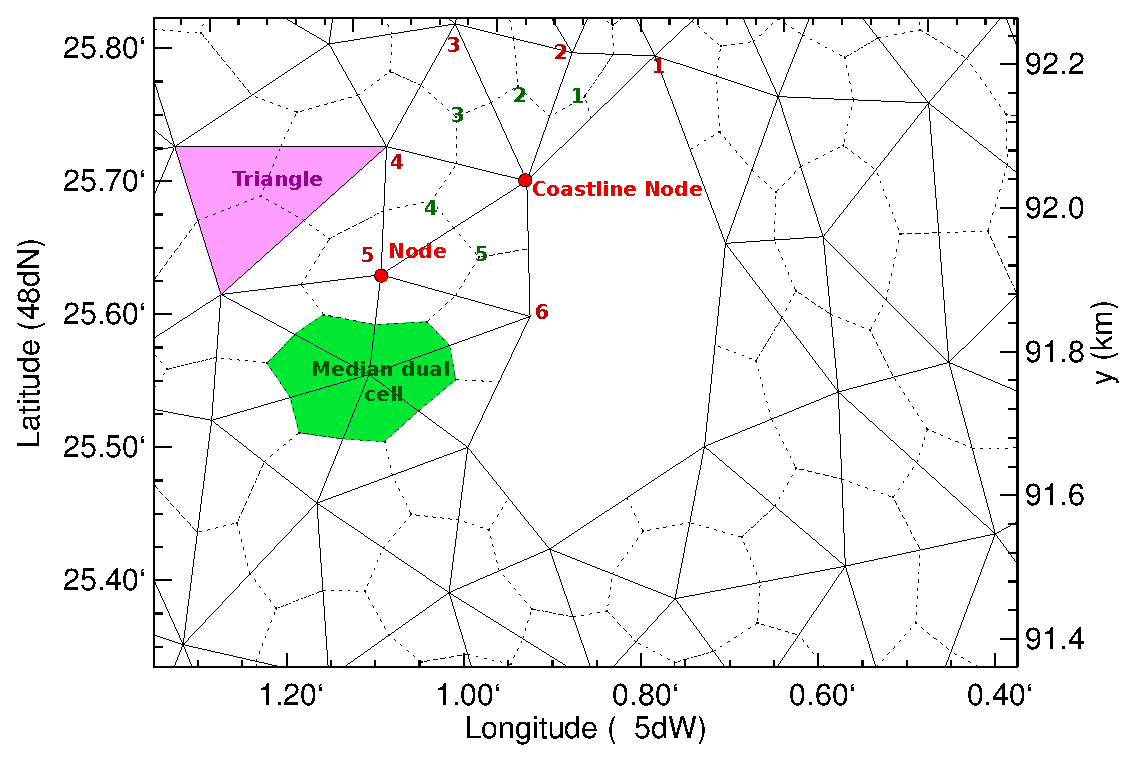
\epsfig{file=./num/grid_triangles.eps,angle=0,width=4.in}
\caption{Example of a region of a triangle-based mesh, with in this case the
 small Island of Bannec, France. If the depth is greater than the minimum
depth, the nodes of the shoreline are active. These are characterized by a
larger number of neighbor nodes (6 in the example chosen) than neighbor
triangles (5 in the same example).}
\label{fig:triangles} \botline
\end{center}
\end{figure}


\vssub
\subsubsection{~Spherical Multiple-Cell (SMC) grid} \label{sub:num_space_SMC}
\opthead{SMC}{\ws (MetOffice)}{J.-G. Li}

\noindent
The Spherical Multiple-Cell (SMC) grid\footnote{~Presently this grid is
activated by a compile switch and can only be used as a stand-alone grid. This
will become a run time option in upcoming model versions.}  \citep{art:Li11}
is an extension of the Cartesian multiple-cell grid \citep{art:Li03} onto the
spherical coordinate system. It is an unstructured grid but retains the
conventional lat-lon grid cells so that all propagation formulations on the
spherical coordinates are still applicable on the SMC grid and hence do all
the finite difference schemes. The SMC grid relaxes the CFL restriction at
high latitudes in a similar fashion as the reduced grid
\citep{art:RA94}. Polar cells are introduced to remove the polar singularity
of the differential transport equation by switching to an integral
equation. The upstream non-oscillatory 2nd order (UNO2) advection schemes
\citep{art:Li08} is implemented on the SMC grid for both spatial and
inter-spectral propagation. A simple rotation scheme is used for wave refraction 
induced rotation and the great circle turning \citep{art:Li12}.  The refraction
scheme is unconditionally stable for any time step but the maximum refraction 
induced rotation angle is limited by the maximum possible refraction angle 
towards the local gradient direction.  Diffusion term similar to the 
\cite{art:BH87} for alleviation of the garden sprinkler effect is used but
the diffusion coefficient is simplified to a single homogeneous parameter
($D_{nn}$ as in Eq.~(\ref{eq:Dnn_d})).  Reduction of computing time with this
new grid is significant in comparison with the conventional grid, thanks to
the relaxed time step restriction at high latitudes and removal of land points
from the model. A remedy for the invalided scalar assumption at high latitude
is provided to extend the global wave model into the entire Arctic Ocean.

The SMC grid can be used for replacing the regular lat-lon grid so that the
model domain can be extended to high latitudes or even the North Pole without
reducing the time step. This application requires little changes to the
regular grid model except for preparing a few extra input files, including the
cell array and face array files. The cell array can be generated with the
existing regular grid bathymetry by using the sea points only and merging
cells in the longitudinal directions at a few latitude steps \citep{art:Li11}.

Another important use of the SMC grid is for multi-resolution grids.
The base level SMC grid cell can be refined into 4 quarterly cells
by halving both the longitude and latitude grid lengths. Any cell
on this refined level can be further divided into another 4 quarterly
cells. This refinement can go on as required, resulting in multi-resolution
grids in a few refined levels. For consistency, the single resolution
SMC grid is considered to have only one level. Wind forcing will remain
to be at the base level resolution for all SMC grids (one level or
multi-level) and it will be interpolated on to the refined levels
(if any) inside the WW3 model. The normal regular grid input files,
such as the water depth, land-sea masks, and sub-grid obstruction,
are also required at present. 

\begin{figure}
\centerline{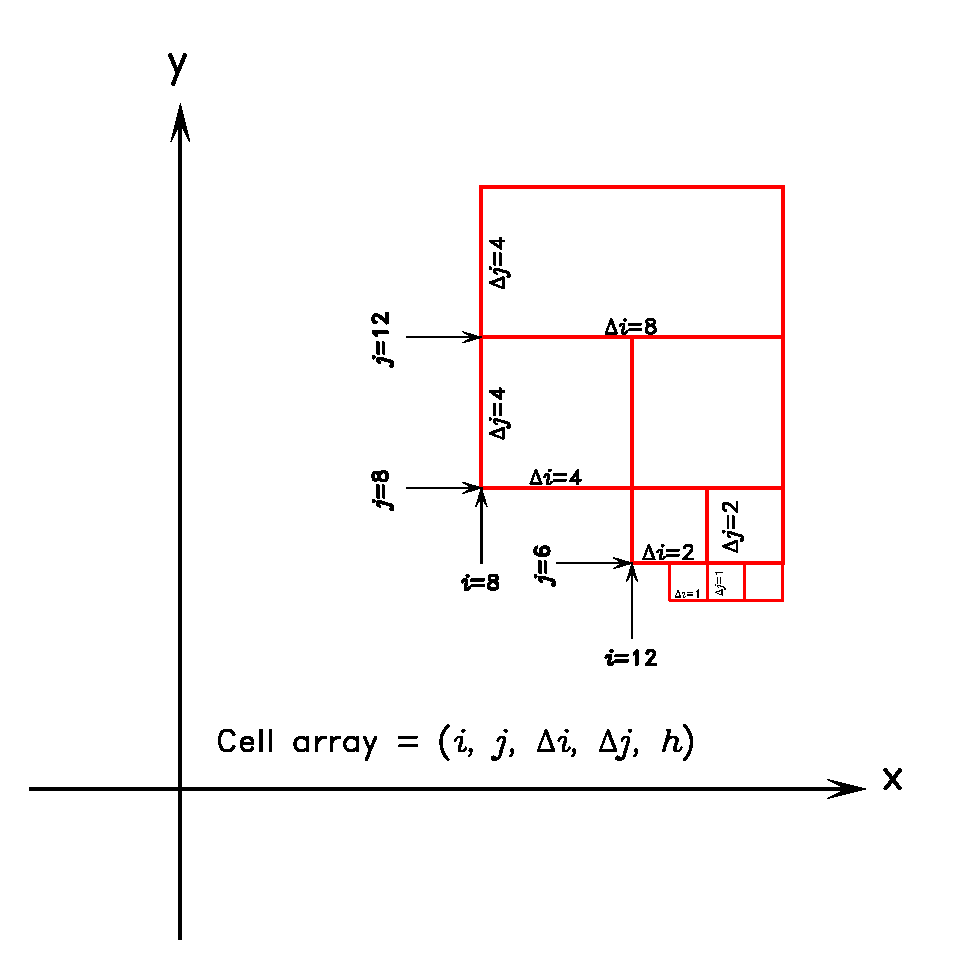
\epsfig{file=./num/smcelary.eps,angle=0,width=3.in}}
\caption{Illustration of cell arrays used in the SMC grid.}
\label{fig:SMCells} \botline
\end{figure}

One important feature of the SMC grid is that it is an unstructured grid, that
is, the cells are not required to be listed side by side as in their physical
position. For the convenience of multi-resolution SMC grid, the cells are
sorted by their sizes so that cells on one given level are grouped together in
one sub-loop for a shared sub-time-step.  The base level time step is halved
as the grid length for the refined level sub-step. This effectively avoids the
model to be slowed down by the refined cells due to their CFL
restrictions. Neighboring cells information for propagation schemes are
provided with cell face arrays, which are pre-calculated for the given cell
array list. So there is no need to expand the sea point only SMC grid cells
onto a full grid for propagation. Figure~\ref{fig:SMCells} illustrates how SMC
cell arrays are defined and Fig.~\ref{fig:SMC_Arctic} shows the Arctic region
in a 6-12-25 km three level SMC grid. The golden and red circles mark the
global and Arctic parts in the SMC6-25 grid. The Arctic part within the golden
circle requires a fixed reference direction to define its wave directional
bins. The global part (upto the golden circle) can be run independently
without the Arctic part. The 4 rows from the red to the golden circles are
duplicated in the Arctic part as boundary cells if the Arctic part is
activated with the ARC option. Separate cell and face arrays are used for the
Arctic part and they are merged into the global ones within the wave model for
propagation.

\begin{figure}
\centerline{\epsfig{file=./num/JCP_Fig2_GArc.eps,angle=0,width=4.in}}
\caption{The Arctic region in a 6-12-25km multi-resolution SMC grid.}
\label{fig:SMC_Arctic} 
\botline
\end{figure}

Some IDL and F90 programs have been developed for generation of SMC grid cell
and face arrays and visualization of the grid mesh and wave fields but they
have not been formally included in the WW3 package yet. An IDL program 
(Glob50SMCels.pro) is provided in aux/smc/SMCG\_TKs/ to generate a global 50km 
SMC grid using a 50km regular grid bathymetry ASCII input file (G50kmBathy.dat). 
Face array generation is done with two F90 programs, one for the global part 
(G50SGlSide.f90) and one for the Arctic part (G50SAcSide.f90).  Due to the special 
treatment of the polar cell \citep{art:Li12}, face arrays for the Arctic polar cell 
requires a different approach than other cells. The face array file has to be 
sorted with a simple Linux script (countcells) before it is fed into the face array 
generation program.  The face arrays also need to be sorted with a Linux script 
(countijsd) to determine the multi-level sub-loop counts.  An independent spectral 
propagation test (G50SMCSRGD.f90) can be run to test the cell and face arrays and 
the its output can be visulised with an IDL script, g50smstrspb.pro, which uses the 
saved projection files from the SMC grid visualization program, g50smcgrids.pro. 
By modifying the projection parameters in g50smcgrids.pro, users can choose a 
projection view point (in lat-lon degree) and save the projection for model 
output visualization.

Compilation of the SMC grid option is similar to that for the regular
lat-lon grid except for that the SMC switch is substituted for the
PR2 UNO combination switches. Note that the SMC grid is built inside
the regular lat-lon grid type so regular lat-lon grid parameters,
such as NX, NY, SX, SY, X1, and Y1, are still required for SMC grid
in ww3\_grid.inp file at the base resolution level. The regular lat-lon
grid water depth, land-sea masks, and sub-grid obstruction input files
are also required and are set at the SMC grid base resolution level.
Due to the merges at high latitudes and refined resolutions if any,
these regular grid input files are modified slightly for consistency
with the SMC grid cells. An IDL program (G50SMCDepth.pro) is an example 
program to generated the regular grid input files for the 50km global 
SMC grid. Refer to the regression test \emph{regtests/ww3\_tp2.10}
for an example of a 3-level SMC grid model for the Lake Erie.

Output for the SMC grid can be processed by the ww3\_outf program
as either the fully expanded regular lat-lon grid output at the base
resolution level or as ASCII out at all SMC grid cell points (type-4).
The regular grid format output can be viewed as other regular grid
output but the refined resolution cells have been converted into 
corresponding base resolution cells for a multi-resolution grid. 
The all cell ASCII output gives field values at the cell centre
so its resolution conforms with the SMC grid. Visulisation of the
all cell ASCII output can done with the aid of the input cell array
file because the output cell sequency is the same as the input cell
array. The IDL script g50smcswhglb.pro is an example program to plot
the global 50km SMC grid SWH output. It uses the projection files
produced by g50smcgrids.pro. Users are encouraged to develop their
own grid-generating and post-processing programs in other languages.

It is recommended to read the model/aux/SMC\_Grid\_Guide.pdf for
more information or to contact \url{Jian-Guo.Li@metoffice.gov.uk} 
for any help about the SMC grid.


\vsssub
\subsubsection{~The Garden Sprinkler Effect} \label{sub:num_GSE}
\vsssub

\noindent
The higher-order accurate propagation schemes are sufficiently free of
numerical diffusion for the so-called `Garden Sprinkler Effect' (GSE) to
occur, i.e., a continuous swell field disintegrates into a set of discrete
swell fields due to the discrete description of the spectrum
\citep[Fig.~3c]{art:BH87}. Several GSE alleviation methods are available in
\ws, as described in the following sections.

\addcontentsline{toc}{subsubsection}{\strut \hspace{24mm} No GSE alleviation}

\vspace{\baselineskip}
\vspace{\baselineskip}
\noindent {\bf No GSE alleviation}

\opthead{PR0 / PR1}{\ws}{H. L. Tolman}

\noindent
In case of no propagation (switch {\code PR0}) or for the first-order
propagation scheme in a traditional or curvilinear grid no GSE alleviation is
available or needed.
\pb
\addcontentsline{toc}{subsubsection}{\strut \hspace{24mm} Booij and Holthuijsen 1987}

\vspace{\baselineskip} 
\vspace{\baselineskip} 
\noindent {\bf Booij and Holthuijsen 1987}

\opthead{PR2}{\ws}{H. L. Tolman}


The classical GSE alleviation method is from \cite{art:BH87}, who derived an
alternative propagation equation for the discrete spectrum, including a
diffusive correction to account for continuous dispersion in spite of the
discrete spectral description. This correction influences spatial propagation
only, which for general spatial coordinates $(x,y)$ becomes

% ------ Correction linear dispersion --------- %
% eq:d_bal_0         Booij and Holthuijsen, 1987
% eq:Dxx
% eq:Dyy
% eq:Dxy
% eq:Dss
% eq:Dnn

\begin{equation}
\frac{\p \cN}{\p t} +
\frac{\p}{\p x} \left [ \dot{x} \cN 
           - D_{xx} \frac{\p \cN}{\p x} \right ] +
\frac{\p}{\p y} \left [ \dot{y} \cN 
           - D_{yy} \frac{\p \cN}{\p y} \right ] -
2 D_{xy} \frac{\p^2 \cN}{\p x \p y} = 0
\: , \label{eq:d_bal_0}\end{equation}  \begin{equation}
D_{xx} = D_{ss} \, \cos^2 \theta + D_{nn} \, \sin^2 \theta
\: , \label{eq:Dxx} \end{equation} \begin{equation}
D_{yy} = D_{ss} \, \sin^2 \theta + D_{nn} \, \cos^2 \theta
\: , \label{eq:Dyy} \end{equation}  \begin{equation}
D_{xy} = ( D_{ss} - D_{nn} ) \, \cos \theta \, \sin \theta
\: , \label{eq:Dxy} \end{equation} \begin{equation}
D_{ss} = (\Delta c_g )^2 \: T_s / 12
\: , \label{eq:Dss} \end{equation} \begin{equation}
D_{nn} =  ( c_g \Delta \theta )^2 \: T_s / 12
\: , \label{eq:Dnn} \end{equation}

\noindent
where $D_{ss}$ is the diffusion coefficient in the propagation direction of
the discrete wave component, $D_{nn}$ is the diffusion coefficient along the
crest of the discrete wave component and $T_s$ is the time elapsed since the
generation of the swell. In the present fractional step method the diffusion
can be added as a separate step

% eq:d_bal_1         Separated diffusion equation

\begin{equation}
\frac{\p \cN}{\p t} = 
\frac{\p}{\p x} \left [ D_{xx} \frac{\p \cN}{\p x} \right ] +
\frac{\p}{\p y} \left [ D_{yy} \frac{\p \cN}{\p y} \right ] +
   2 D_{xy} \frac{\p^2 \cN}{\p x \p y}
\: . \label{eq:d_bal_1} \end{equation}

\noindent
This equation is incorporated with two simplifications, the justification of
which is discussed in \cite{tol:OMB95}. First, the swell `age' $T_s$ is kept
constant throughout the model (defined by the user, no default value
available). Secondly, the diffusion coefficients $D_{ss}$ and $D_{nn}$ are
calculated assuming deep water

% eq:Dss_d
% eq:Dnn_d

\begin{equation}
D_{ss} = \left ( \: (X_\sigma-1) \: \frac{\sigma_m}{2 k_m} \right )^2
\: \frac{T_s}{12} \: , \label{eq:Dss_d} \end{equation} \begin{equation}
D_{nn} =  \left ( \frac{\sigma_m}{2 k_m} \Delta \theta \right )^2
\: \frac{T_s}{12} \: , \label{eq:Dnn_d} \end{equation}

\noindent
where $X_\sigma$ is defined as in Eq.~(\ref{eq:sigma_grid}). With these two
assumptions, the diffusion tensor becomes constant throughout the spatial
domain for each separate spectral component.

Equation~(\ref{eq:d_bal_1}) is solved using a forward-time central-space
scheme. At the cell interface between points $i$ and $i-1$ in $\phi$ ($x$)
space, the term in brackets in the first term on the right side of
Eq.~(\ref{eq:d_bal_1}) (denoted as $\cD_{i,-})$ is estimated as

% eq:ddif_1          Discrete diffusion 1

\begin{equation}
D_{xx} \frac{\p \cN}{\p x} \approx \cD_{i,-} =
\left . D_{xx} \; \left ( \frac{\cN_i - \cN_{i-1}}{\Delta x} \right ) \: 
\right |_{j,l,m} \: . \label{eq:ddif_1} \end{equation}

\noindent
Corresponding values for counters $i$ and $i+1$, and for gradients in
$\lambda$ ($y$) space again are obtained by rotating indices and
increments. If one of the two grid points is located on land,
Eq.~(\ref{eq:ddif_1}) is set to zero. The mixed derivative at the right side
of Eq.~(\ref{eq:d_bal_1}) (denoted as $\cD_{ij,--}$) is estimated for the grid
point $i$ and $i-1$ in $x$-space and $j$ and $j-1$ in $y$-space as

% eq:ddif_2          Discrete diffusion 2

\begin{equation}
\cD_{ij,--} = \left . \: D_{xy} 
\left ( \frac{- \cN_{i,j} + \cN_{i-1,j} +
              \cN_{i,j-1} - \cN_{i-1,j-1}}
           {0.5 ( \Delta x_j + \Delta x_{j-1} ) \: \Delta y}
              \right ) \: \right |_{l,m} 
\: . \label{eq:ddif_2} \end{equation}

\noindent
Note that the increment $\Delta x$ is a function of $y$ due to the use of the
spherical grid. This term is evaluated only if all four grid points considered
are sea points, otherwise it is set to zero. Using a forward in time
discretization of the first term in Eq.~(\ref{eq:d_bal_1}), and central in
space discretizations for the remainder of the first and second term on the
right side, the final algorithm becomes

% eq:ddif_3          Discrete diffusion 3

\begin{eqnarray}
\cN_{i,j,l,m}^{n+1} = \cN_{i,j,l,m}^n + 
\frac{\Delta t}{\Delta x} 
   \left ( \cD_{i,+} - \cD_{i,-} \right ) +
\frac{\Delta t}{\Delta y}
   \left ( \cD_{j,+} - \cD_{j,-} \right ) \nonumber \\
+ \frac{\Delta t}{4} \left ( \cD_{ij,--} + 
   \cD_{ij,-+} + \cD_{ij,+-} + \cD_{ij,++} \right )
\: . \label{eq:ddif_3} \end{eqnarray}

\noindent
Stable solutions are obtained for \citep[e.g.,][Part I section
7.1.1]{bk:Fle88}

% eq:ddif_4          Stability

\begin{equation}
\frac{D_{\max} \: \Delta t}{\min(\Delta x , \Delta y)^2}
\leq 0.5 \: , \label{eq:ddif_4} \end{equation}

\noindent
where $D_{\max}$ is the maximum value of the diffusion coefficient (typically
$D_{\max} = D_{nn}$). Because this stability criterion is a quadratic function
of the grid increment, stability can become a serious problem at high
latitudes for large scale applications. To avoid this putting undue
constraints on the time step of a model, a corrected swell age $T_{s,c}$ is
used

% eq:Ts_cor

\begin{equation}
T_{s,c} = T_s \min \left \{ \: 1 \: , \: 
\left ( \frac{\cos(\phi)}{\cos(\phi_c)} \right )^2 \: \right \}
\: , \label{eq:Ts_cor} \end{equation}

\noindent
where $\phi_c$ is a cut-off latitude defined by the user.

\vspace{\baselineskip} \noindent
 
The above diffusion is needed for swell propagation, but is not realistic
for growing wind seas. For wind seas, the \uq\ scheme without the
dispersion correction is sufficiently smooth to render stable fetch-limited
growth curves \citep{tol:OMB95}. To remove minor oscillations, a small
isotropic diffusion is used for growing wave components. To assure that this
diffusion is small and equivalent for all spectral components, it is
calculated from a preset cell Reynolds (or cell Peclet) number $\cR = c_g
\Delta x D_g^{-1} = 10$, where $D_g$ is the isotropic diffusion for growing
components

% eq:Dg              Diffusion growing components

\begin{equation}
D_g = \frac{c_g \: \min(\Delta x , \Delta y)}{\cR} \: . \label{eq:Dg}
 \end{equation}

\noindent
The diffusion for swell and for wind seas are combined using a linear
combination depending on the nondimensional wind speed or inverse wave age
$u_{10} c^{-1} = u_{10} k \sigma^{-1}$ as

% eq:Xg              Linear combination for diffusion
% eq:Dss_f           Final Dss
% eq:Dnn_f           Final Dnn

\begin{equation}
X_g = \min \: \left \{ \: 1 \: , \: \max \: \left [ \: 0 \: , \:
3.3 \left ( \frac{k \, u_{10}}{\sigma} \right ) - 2.3
\: \right ] \: \right \}
 \: , \label{eq:Xg} \end{equation} \begin{equation}
D_{ss} = X_g D_g + (1-X_g) D_{ss,p}
\: , \label{eq:Dss_f} \end{equation} \begin{equation}
D_{nn} = X_g D_g + (1-X_g) D_{nn,p}
\: , \label{eq:Dnn_f} \end{equation}

\noindent
where the suffix $p$ denotes propagation diffusion as defined in
Eqs.~(\ref{eq:Dss_d}) and (\ref{eq:Dnn_d}). The constants in Eqs~(\ref{eq:Dg})
and (\ref{eq:Xg}) are preset in the model.


\pb
\addcontentsline{toc}{subsubsection}{\strut \hspace{24mm} Spatial averaging}

\vspace{\baselineskip} 
\vspace{\baselineskip} 
\noindent {\bf Spatial averaging}

\opthead{PR3}{\ws}{H. L. Tolman}


The major drawback of the above GSE alleviation method is its potential impact
on model economy as discussed in relation to Eq.~(\ref{eq:ddif_4}) and in
\cite{tol:Waves01a,tol:OMOD02b}. For this reason, an alternative additional GSE alleviation
method has been developed for \ws.

This method which represents the default for \ws, replaces the
additional diffusion step (\ref{eq:d_bal_1}) with a separate fractional step
in which direct averaging of the field of energy densities for a given
spectral component is considered. The area around each grid point over which
the averaging is performed extends in the propagation ($\bs$) and normal
($\bn$) directions as

\begin{equation}
\pm \gamma_{a,s} \: \Delta c_g \: \Delta t \: \bs \:\:\: ,
\pm \gamma_{a,n} \: c_g \Delta \theta \: \Delta t \: \bn \:\:\: , \label{eq:GSE_avg}
\end{equation}

\noindent
where $\gamma_{a,s}$ and $\gamma_{a,n}$ are tunable constants, the default
value of which is set to 1.5. This averaging is illustrated in
Fig.~\ref{fig:GSE_1}. Note that these values may require some retuning for
practical applications, as discussed in \cite{tol:OMOD02b}. Appendix A of the
latter paper presents details of the averaging scheme, including conservation
considerations. Consistency with the \cite{art:BH87} approach furthermore
implies that $\gamma_{a,s}$ and $\gamma_{a,n}$ should vary with the spatial
grid resolution \citep[see][Appendix]{tol:OMOD08a}.

Note that this kind of averaging with dominant directions $\bs$ and $\bn$ is
similar to the \cite{art:BH87} diffusion method, that uses the same main
directions. The averaging method, however, never influences the time step,
because it is completely separated from the actual propagation. Moreover, if
explicit schemes are used with typically $c_g \Delta t / \Delta x < 1$, it is
obvious that the averaging over the area as defined in (\ref{eq:GSE_avg}) will
generally require information at directly neighboring spatial grid points
only, as in Fig.~\ref{fig:GSE_1}. Furthermore, this method does not require
high-latitude filtering.

\begin{figure} \begin{center}
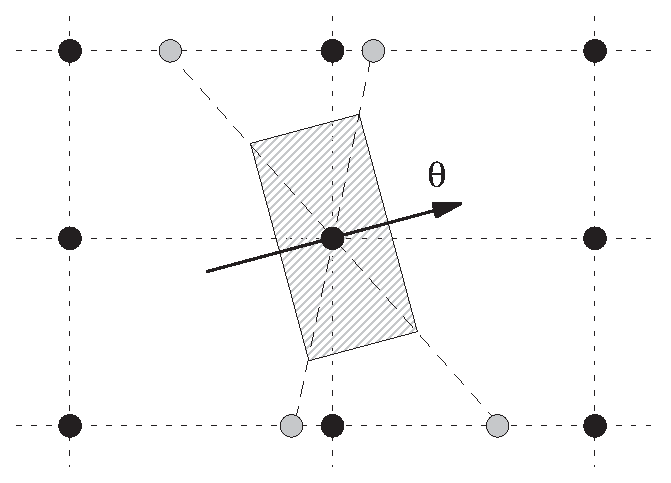
\epsfig{file=./num/GSE_1.eps,angle=0,width=2.2in}
\caption{Schematic of spatial averaging GSE alleviation technique. 
Solid circles and dotted lines represent the spatial grid. Hatched
area represent averaging area to be considered. Corner point values are
obtained from the central grid point and the gray points. The latter values
are obtained by interpolation from adjacent grid points
\citep[from][]{tol:OMOD02b}.}
\label{fig:GSE_1} \botline
\end{center}
\end{figure}

As is illustrated in \cite{tol:OMOD02b,tol:OMB02b}, this method gives
virtually identical results as the previous method, but does so at slightly
lower costs. For high-resolution applications, the averaging method may become
dramatically more economical.



Finally, the GSE can be alleviated somewhat by assuring that the discrete
spectral directions do not coincide with spatial grid lines. This can be
achieved by defining the first discrete direction $\theta_1$ as

% eq:theta1          First direction

\begin{equation}
\theta_1 = \alpha_\theta \: \Delta \theta \:\:\: , \label{eq:theta1}
\end{equation}

\noindent
where $-0.5 \leq \alpha_\theta \leq 0.5$ can be defined by the user. Note that
setting $\alpha \neq 0$ is beneficial to the first-order scheme, but has
negligible impact on the third-order scheme.
 

\pb
\vsssub
\subsubsection{~Unresolved obstacles} \label{sub:num_obst}
\conthead{\ws}{H. L. Tolman}

\noindent
Even at the time of the original tuning of \ws\ version 1.15
\citep{tol:OMB02a}, it was clear that unresolved islands groups are a major
source of local wave model errors. This was illustrated in some more detail in
\citet[][Fig.~3]{tol:Waves01a}, and \citet[][Fig.~8]{tol:WaF02}. In \ws, a
methodology from \swan\ \citep{art:BRH99,man:SWAN3} was adopted to apply the
effects of unresolved obstacles at the cell boundaries of the spatial grid
within the numerical scheme. In this approach, the numerical fluxes between
cells through their common boundary are suppressed according to the degree of
obstruction provided by the unresolved obstacle. In this approach, the
numerical propagation scheme of the \uq\ scheme of Eq.~(\ref{eq:uq_xy_tot}) is
modified as

% eq:uq_xy_obstr

\begin{equation}
\cN_{i,j,l,m}^{n+1} = \cN_{i,j,l,m}^n +
\frac{\Delta t}{\Delta \phi} \left [ \alpha_{i,-} \cF_{i,-} - \alpha_{i,+} \cF_{i,+} \right ]
\: . \label{eq:uq_xy_obstr} \end{equation}

\begin{figure} \begin{center}
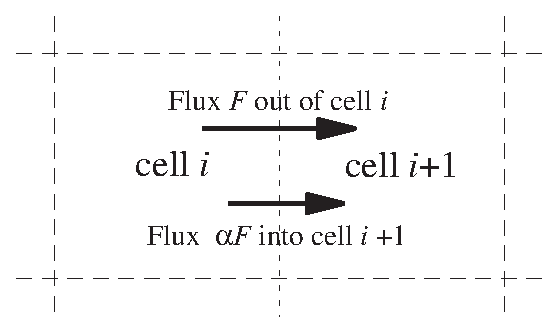
\epsfig{file=./num/obstr.eps,angle=0,width=2.2in}
\caption{Graphical depiction of treatment of unresolved obstacles. Common cell
         boundary (dotted line) has transparency $\alpha$. Dashed lines
         represent other cell boundaries. Numerical flux from left to right.}
         \label{fig:obstr} \botline
\end{center}
\end{figure}

\noindent
where $\alpha_{i,-}$ and $\alpha_{i,+}$ are `transparencies' of the
corresponding cell boundaries, ranging from 0 (closed boundary) to 1 (no
obstructions). For outflow boundaries, transparencies by definition are 1,
otherwise energy will artificially accumulate in cells. For inflow boundaries,
transparencies less than 1 result in elimination of obstructed energy at the
cell boundary. This approach is graphically depicted in
Fig.~\ref{fig:obstr}. Note that a similar approach is easily adopted in the
first and second order schemes.  Note, furthermore, that an alternate
obstruction approach with obstructions as a function of the spectral direction
$\theta$ has been used by \cite{art:HY96} and \cite{art:HMM00}.

Two methods for defining the obstructions are available in the model. The
first defines the obstructions directly at the grid boundary. This requires
the generation of staggered depth-transparency grids. The second allows the
user to define depths and transparencies at the same grid. In this case, the
transparency at the inflow boundary becomes $0.5(1+\alpha_i)$, and the outflow
transparency by definition is 1. To complete the total transparency
$\alpha_i$, the next cell in the flow direction will have an inflow
transparency $2\alpha_i/(1+\alpha_i)$. If consecutive cells are partially
obstructed, the product of individual transparencies is applied.

This approach can also be used to continuously model the effects of ice
coverage on wave propagation. This is discussed in \para\ref{sub:num_ice}.
Details of the sub-grid treatment of islands and ice can be found in
\cite{tol:OMOD03a}. A study of impacts of this approach in large scale wave
models is presented in \cite{tol:OMB02b,tol:OMOD03a}.

The default setting of \ws\ is not to include sub-grid modeling of
obstacles. Generating obstruction grids can be labor intensive. For this
reason, an automated approach for generating bottom and obstruction grids was
developed by \cite{tol:MMAB07a, tol:OMOD08a}.  Note that this option does not
involve compile-level choices, but is entirely controlled from the grid
preprocessor (see following chapter).


\vsssub
\subsubsection{~Continuously moving grids} \label{sub:num_move}
\opthead{MGx}{\ws}{H. L. Tolman}

\addcontentsline{toc}{subsubsection}{\strut \hspace{24mm} General concepts}

\noindent {\bf General concepts}
\vspace{\baselineskip} 
\noindent
In order to address wave growth issues in rapidly changing, small scale
conditions such as hurricanes, an option to add a given continuous advection
speed to the grid has been added to the model in model version 3.02. This
model version is described in detail in \cite{tol:OMOD05b}. Here, only a
cursory description is given.

\begin{center}
\rule[1mm]{55mm}{1.0mm} WARNING \rule[1mm]{55mm}{1.0mm} \\
 \vspace{\baselineskip}
\parbox{120mm}{The continuously moving grid version of \ws\ is only intended 
for testing wave model properties in highly idealized conditions. This model
version should only be used for deep water without mean currents and land
masses. Furthermore, to avoid complications with great circle propagation,
only Cartesian grid should be used. The option is furthermore implemented only
for propagation options {\F pr1} and {\F pr3}. Note that this is not checked
in the scripts or programs at either the compile or run time level.  This
option is not described in the body of the manual but in this appendix only,
because it is not considered to be a general application.} \\
\vspace{\baselineskip}
\rule[1mm]{55mm}{1.0mm} WARNING \rule[1mm]{55mm}{1.0mm}
\end{center}

\noindent
For the above described application Eq.~(\ref{eq:bal_plane}) can be written as

\begin{equation}
\frac{\partial N}{\partial t} + 
\left ( {\bf\dot{x}}-{\bf{v}}_g \right ) \cdot \nabla_x N  = 
\frac{S}{\sigma} \: , \label{eq:bal_move}
\end{equation}

\noindent
where ${\bf{v}}_g$ represents the advection velocity of the grid. This option
is selected when compiling the model (see below). A second compile level
option allows for adding the grid advection velocity ${\bf{v}}_g$ to the wind
field. This allows for a simple method to assure mass conservation of a wind
field independent of the actual and instantaneous grid advection velocity. The
advection velocity ${\bf{v}}_g$ can vary in time and is provided by the user
at the run time of the model (see below).

\vspace{\baselineskip} 
\vspace{\baselineskip} 
\addcontentsline{toc}{subsubsection}{\strut \hspace{24mm} Numerical implementation}
\noindent {\bf Numerical implementation}
\vspace{\baselineskip} 

\noindent
For the simplified conditions for which Eq.~(\ref{eq:bal_move}) is valid, the
implementation of the moving grids is trivial if it is considered that this
equation is equivalent to

\begin{equation}
\frac{\partial N}{\partial t} + 
\nabla_x \cdot \left ( {\bf\dot{x}}-{\bf{v}}_g \right ) N  = 
\frac{S}{\sigma} \: , \label{eq:bal_move2}
\end{equation}

\noindent
which in turn implies that the advection velocity ${\bf{v}}_g$ can be added
directly to ${\bf\dot{x}}$ for arbitrary numerical schemes solving
Eq.~(\ref{eq:bal_plane}). Because this influences the net advection velocity,
it also influences stability characteristics. This impact has been accounted
for automatically by including the moving grid velocity in the calculation of
the actual propagation time step in Eq~(\ref{eq:dtpl}). Hence, the user need
to provide a proper maximum propagation time step representative for $\bf{v}_g
= 0$ only.

The motion of the grid has an apparent influence on the Garden Sprinkler
Effect (GSE), due to the different retention time in the grid of spectral
components with identical frequency but different propagation direction.
Current GSE alleviation methods tend to be more efficient for younger swells
than for older swells. Hence, swells with longer retention time in the moving
grid tend to show a more pronounced GSE \citep[see][]{tol:OMOD05b}. To
mitigate this apparent imbalance in GSE alleviation,  Eq.~(\ref{eq:GSE_avg}) is
replaced with

\begin{equation}
\pm \gamma_a \gamma_{a,s} \: \Delta c_g \: \Delta t \: \bs \:\:\: ,
\pm \gamma_a \gamma_{a,n} \: c_g \Delta \theta \: \Delta t \: \bn \:\:\: ,
\label{eq:move_GSE_avg1}
\end{equation}

\begin{equation}
\gamma_a = \left ( \frac{|\dot{\bf{x}}|}{|\dot{\bf{x}}-\bf{v}_g|}
\right ) ^{p}
\label{eq:move_GSE_avg2}
\end{equation}

\noindent
where $\gamma_a$ is a correction factor accounting for the grid movement, and
where the power $p$ is a parameter allows for some tuning. With this
modification, the effects of the GSE can be distributed more evenly over the
grid by rescaling the amount of smoothing applied with the expected residence
time of corresponding spectral component in the moving grid
\citep[see][]{tol:OMOD05b}.

\vspace{\baselineskip} 
\vspace{\baselineskip} 
\addcontentsline{toc}{subsubsection}{\strut \hspace{24mm} Running with moving grids}
\noindent {\bf Running with moving grids}
\vspace{\baselineskip} 

\noindent
To switch on the moving of the grid, or the correction of the wind field, two
optional switches are added to the \ws\ source code:

\begin{slist}
\sit{mgp} {Apply advection correction for continuous moving grid.}
\sit{mgw} {Apply wind correction for continuous moving grid.}
\sit{mgg} {Apply correction to averaging strength in GSE correction for
           continuous moving grid.}
\end{slist}

\noindent
The advection velocity and direction is input to the shell similar to the
input of homogeneous currents (see bottom of file {\file ww3\_shel.inp} in
section~\ref{sec:ww3shel}), exchanging the keyword '{\code CUR}' with '{\code
  MOV}'. The advection velocity can be changed in time like all homogeneous
input fields. An example of running with a moving grid model is given in test
case {\file ww3\_ts3}. A similar capability exist in {\file ww3\_multi.inp} in
section \ref{sec:ww3multi}, and is tested in test case {\file mww3\_test\_05}.

\vssub
\subsubsection{~Rotated grids} \label{sub:num_space_rotagrid}
\opthead{RTD}{\ws\ (MetOffice)}{J.-G. Li}

\noindent
Rotated grid is a latitude-longitude (lat-lon) grid and is obtained by
rotating the North Pole to a new pole position at latitude $\phi_{p}$ and
longitude $\lambda_{p}$ in the standard latitude-longitude system.  The new
pole position is chosen so that an interested model domain may be placed
around the rotated equatorial area for a evenly spaced lat-lon mesh. For this
reason the rotated grid is also known as \emph{Equatorial grid}. For instance,
the North Atlantic and European wave (NAEW) model used in the UK Met Office
uses a rotated pole at 37.5N, 177.5E so that London, UK
(\textasciitilde{}51.5N 0.0E) is almost on the rotated equator. This rotated
grid allows a much more evenly spaced lat-lon mesh in the NAE domain than the
standard lat-lon grid in the same area. In \ws\, the rotated grid is
implemented with minimum changes to the original lat-lon grid. In fact, the
rotated grid is treated just like the standard lat-lon grid inside the
model. Only input and output files are modified for the rotated grid. Users
should choose the regular lat-lon grid along with the RTD switch to use the
rotated grid. Model input files, like wind, current and ice files should be
mapped on to the rotated grid. For convenience of nesting in standard lat-lon
grid, boundary conditions for the rotated grid use standard lat-lon grid
points, which are converted into rotated grid lat-lon inside \ws\. List of 2D
spectral output locations in ww3\_shel.inp are also specified in standard
lat-lon. All directional output such as wind direction, peak direction, 2D
spectra, etc. are converted into standard lat-lon orientation. Full grid
output are still on rotated grid but 2D spectra locations have been converted
into standard lat-lon.

Four subroutines are provided in module {\bf w3servmd.ftn} for rotated grid
conversion:
\begin{vlist}
\vit{w3spectn}{}{Turns wave spectrum anti-clockwise by AnglD}
\vit{w3acturn}{}{Turns wave action(k,nth) anti-clockwise by AnglD}
\vit{w3lltoeq}{}{Convert standard into rotated lat/lon plus AnglD}
\vit{w3eqtoll}{}{Reverse of w3lltoeq, but AnglD unchanged}
\end{vlist}
These subroutines are self-contained and can be extracted outside the model
for pre- or post-processing of rotated grid files. Some conversion tools have
been developed based on these subroutines but have not been included in \ws\
yet. Refer to the regression test \emph{regtests/ww3\_tp2.11} for an example
of a rotated grid model (NAEW) and the document \emph{RotatedGrid.pdf} for
rotated grid formulations. For more information, users may contact
\url{Jian-Guo.Li@metoffice.gov.uk}.

\vssub
\subsection{~Intra-spectral propagation} \label{sub:spec}
\vssub
\subsubsection{~General concepts}
\vsssub

The third step of the numerical fractional step algorithm considers refraction
and residual (current-induced) wavenumber shifts. Irrespective of the spatial
grid discretization and coordinate system, the equation to be solved in this
step becomes

%-----------------------------------%
% Step : Intra-spectral propagation %
%-----------------------------------%
% eq:step_intra
% eq:k_dot_g

\begin{equation}
\frac{\p N}{\p t} + \frac{\p}{\p k} \, \dot{k}_g N +
\frac{\p}{\p \theta} \, \dot{\theta}_g N = 0
\: , \label{eq:step_intra} \end{equation} \begin{equation}
\dot{k}_g  = \frac{\p \sigma}{\p d} 
    \frac{{\bf U} \cdot \nabla_x d}{c_g}  -
    {\bf k} \cdot \frac{\p {\bf U}}{\p s}
\: . \label{eq:k_dot_g} \end{equation}

\noindent
where $\dot{k}_g$ is the wavenumber velocity relative to the grid, and
$\dot{\theta}_g$ is given by (\ref{eq:theta_g_dot}) and (\ref{eq:theta_dot}).
This equation does not require boundary conditions in $\theta$-space, as the
model by definition uses the full (closed) directional space. In $k$-space,
however, boundary conditions are required. At low wavenumbers, it is assumed
that no wave action exists outside the discrete domain. It is therefore
assumed that no action enters the model at the discrete low-wavenumber
boundary. At the high-wavenumber boundary, transport across the discrete
boundary is calculated assuming a parametric spectral shape as given by
Eq. (\ref{eq:tail_N_k}). The derivatives of the depth as needed in the
evaluation of $\dot{\theta}$ are mostly determined using central
differences. For points next to land, however, one-sided differences using sea
points only are used.

Propagation in $\theta$-space can cause practical problems in an explicit
numerical scheme, as the refraction velocity can become extreme for long waves
in extremely shallow water or due to strong current shears. Similarly, 
the propagation in $k$-space suffers from similar problems in very shallow water. 
To avoid the need of extremely small time steps
due to refraction, the propagation velocities in $\theta$-space and $k$-space
(\ref{eq:theta_dot}) are filtered,

% eq:theta_filter

\begin{equation}
\dot{\theta} = X_{rd}(\lambda,\phi,k)\left( \dot{\theta_d} + 
\dot{\theta_c} + \dot{\theta_g} \right)\: , \label{eq:theta_filter} \end{equation}

\noindent
where the indices d, c and g refer to the depth, current and great-circle
related fraction of the refraction velocity in (\ref{eq:theta_dot}). The
filter factor $X_{rd}$ is calculated for every wavenumber and location
separately, and is determined so that the \cfl\ number for propagation in
$\theta$-space due to the {\em depth} refraction term cannot exceed a pre-set
(user defined) value (default 0.7). This corresponds to a reduction of the
bottom slope for some low frequency wave components. For mid-latitudes, the
effected components are expected to carry little energy because they are in
extremely shallow water. Long wave components carrying significant energy are
usually traveling toward the coast, where their energy is dissipated
anyway. This filtering is also important for short waves, and close to the
pole. The effect of this filter can be tested by reducing the time steps for
intraspectral refraction and by looking at the maximum CFL numbers in the
output of the model.  These are computed just before the filter is applied.

% \vspace{\baselineskip}
% \centerline{\ldots ADD DYNAMIC TIME INTEGRATION \ldots}

\vspace{\baselineskip} \noindent 
The spectral space is always discretized with constants directional increments
and a logarithmic frequency grid (\ref{eq:sigma_grid}) to accommodate
computations of the nonlinear interaction $S_{nl}$. First, second and third
orders schemes are available, and are presented in the following sections.
\vssub
\subsubsection{~First order scheme}
\opthead{PR1}{\ws}{H. L. Tolman}

\noindent
In the first order scheme the fluxes in $\theta$- and $k$-space are calculated
Cf. Eqs. (\ref{eq:1up_xy_1}) through (\ref{eq:1up_xy_3}) (replacing $\cN$ with
$N$ and rotating the appropriate counters). The complete first order scheme
becomes

% eq:1up_intra_tot

\begin{equation}
N_{i,j,l,m}^{n+1} = N_{i,j,l,m}^n 
 + \frac{\Delta t}{\Delta \theta} \left [ \cF_{l,-} - \cF_{l,+} \right ]
 + \frac{\Delta t}{\Delta k_m} \left [ \cF_{m,-} - \cF_{m,+} \right ]
\: , \label{eq:1up_intra_tot} \end{equation}

\noindent
where $\Delta \phi$ is the directional increment, and $\Delta k_m$ is the
(local) wavenumber increment. The low-wavenumber boundary conditions is
applied by taking $\cF_{m,-}=0$ for $m=1$, and the high wavenumber boundary
condition is calculated using the parametric approximation (\ref{eq:tail_N_k})
for N, extending the discrete grid by one grid point to high wavenumbers.
\vssub
\subsubsection{~Second  order scheme (UNO)}
\opthead{UNO}{Met Office}{J.-G. Li}

\noindent
The UNO2 scheme for the directional$\theta$-space is identical to the regular
grid one assuming that the directional bins are regularly spaced. For the
\emph{k}-space, however, the UNO2 scheme uses its irregular version, which
uses local gradients instead of differences to estimate wave action value at
the mid-flux point for the cell face between spectral bin \emph{i}-1 and
\emph{i}, that is:
\begin{equation}
  N_{i-}^{*}=N_{c}+sign\left(N_{d}-N_{c}\right)\frac{\left(\Delta
      k_{c}-|\dot{k}_{i-}|\Delta
      t\right)}{2}\min\left(|\frac{N_{u}-N_{c}}{k_{u}-k_{c}}|,|\frac{N_{c}-N_{d}|}{k_{c}-k_{d}}\right)
  \:\:\: ,
\label{eq:UNO2irregular}
\end{equation}

\noindent
where \emph{i}- is the wave number \emph{k} bin index; the subscripts
\emph{u}, \emph{c} and \emph{d} indicate the \emph{upstream, central} and
\emph{downstream} cells, respectively, relative to the given \emph{i}- face
velocity $\dot{k}_{i-}$; $k_{c}$is the central bin wave number and $\Delta
k_{c}$is the central bin widith. Details of the irregular grid UNO2 scheme are
given in \cite{art:Li08}.

Boundary conditions for the $\theta$-space is the natural periodic
condition. For the \emph{k}-space, two more zero spectral bins are added to
each end of the wave spectral domain as the UNO2 scheme is 2nd order in
accuracy.



\vssub
\subsubsection{~Third  order scheme (UQ)}
\opthead{UQ}{\ws}{H. L. Tolman}

\noindent
The \uq\ scheme for the $\theta$-space is implemented similar to the scheme
for physical space, with the exception that the closed direction space does
not require boundary conditions. The variable grid spacing in $k$-space
requires some modifications to the scheme as outlined by
\cite[{Appendix}]{art:Leo79}. Equations~(\ref{eq:quick_1}) through
(\ref{eq:quick_4}) then become

% ------ QUICKEST scheme for k space---------- %
% eq:quick_1k        Basic flux
% eq:quick_2k        Boundary value
% eq:quick_3k        Divergence
% eq:quick_4k        CFL number

\begin{equation}
\cF_{m,-} = \left [ \dot{k}_{g,b} \: N_b \: \right ]^n_{i,j,l}
\: , \label{eq:quick_1k}\end{equation} \begin{equation}
\dot{k}_{g,b} = 0.5 \: \left ( \dot{k}_{g,m-1} + \dot{k}_{g,m} 
\: \right )  \: , \label{eq:quick_1ak}
\end{equation} \begin{equation}
N_b = \frac{1}{2} \left [ \rule[0mm]{0mm}{\baselineskip} \: 
(1+C)N_{i-1} + (1-C)N_i \: \right ] - \:
\frac{1-C^2}{6} \: {\cal CU} \: \Delta k^2_{m-1/2}, \label{eq:quick_2k} \end{equation} \begin{equation}
{\cal CU} =  \left \{ \begin{array}{ccc}
\frac{1}{\Delta k_{m-1}}
\left [ \frac{N_{ m }-N_{m-1}}{\Delta k_{m-1/2}} - 
        \frac{N_{m-1}-N_{m-2}}{\Delta k_{m,-3/2}} \right ]
               & \mbox{for} & \dot{k}_b \geq 0 \\
\frac{1}{\Delta k_m}
\left [ \frac{N_{m+1}-N_{ m }}{\Delta k_{m+1/2}} -
       \frac{N_{ m }-N_{m-1}}{\Delta k_{m-1/2}} \right ]
               & \mbox{for} & \dot{k}_b   <  0
\end{array} \right . \: , \label{eq:quick_3k}
\end{equation} \begin{equation}
C = \frac{\dot{k}_{g,b} \: \Delta t}{\Delta k_{m-1/2}}
\: , \label{eq:quick_4k} \end{equation}

\noindent
where $\Delta k_m$ is the discrete band or cell width at grid point $m$, and
where $\Delta k_{m-1/2}$ is the distance between grid points with counters $m$
and $m-1$. The \ult\ limiter can be applied as in Eqs.~(\ref{eq:ult_1})
through (\ref{eq:ult_4}), if the \cfl\ number of Eq.~(\ref{eq:quick_4k}) is
used. At the low- and high-wavenumber boundaries the fluxes again are
estimated using a first-order upwind approach, with boundary conditions as
above defined for the first-order scheme. The final scheme in $k$-space
becomes

% eq:1uq_k_tot

\begin{equation}
N_{i,j,l,m}^{n+1} = N_{i,j,l,m}^n 
 + \frac{\Delta t}{\Delta k_m} \left [ \cF_{m,-} - \cF_{m,+} \right ]
\: , \label{eq:uq_k_tot} \end{equation}
\vssub
\subsection{~Non-ice source terms integration} \label{sub:source}
\vssub

Finally, the source terms are accounted for by solving

%---------------------%
% Step : Source terms %
%---------------------%
% eq:step_source

\begin{equation}
\frac{\p N}{\p t} = \cS_{no~ice} \: . \label{eq:step_source}
\end{equation}

\noindent 
As in \wam, a semi-implicit integration scheme is used. In this scheme the
discrete change of action density $\Delta N$ becomes \citep{art:WAM88}

% eq:implicit_st

\begin{equation}
\Delta N(k,\theta) = \frac{\cS(k,\theta)}{1- \epsilon D(k,\theta)\Delta t}
\: , \label{eq:implicit_st} \end{equation}

\noindent 
where $D$ represents the diagonal terms of the derivative of $\cS$ with
respect to $N$ \citep[Eqs. 4.1 through 4.10]{art:WAM88}, and where $\epsilon$
defines the offset of the scheme. Originally, $\epsilon = 0.5$ was implemented
to obtain a second order accurate scheme. Presently, $\epsilon = 1$ is used as
it is more appropriate for the large time steps in the equilibrium range of
the spectrum \citep{pro:HA98,art:HA01}, and as it result in much smoother
integration of the spectrum. The change of $\epsilon$ has little impact on
mean wave parameters, but makes the dynamical time stepping as described below
more economical.

The semi-implicit scheme is applied in the framework of a dynamic
time-stepping scheme \citep{tol:JPO92}. In this scheme, integration over the
global time step $\Delta t_g$ can be performed in several dynamic time steps
$\Delta t_d$, depending on the net source term $\cS$, a maximum change of
action density $\Delta N_m$ and the remaining time in the interval $\Delta
t_g$. For the $n^{\rm th}$ dynamic time step in the integration over the
interval $\Delta t_g$, $\Delta t_d^n$ is calculated in three steps as

% ------ Dynamic s.t. int. scheme ------- %
% eq:st_d_1
% eq:st_d_2a
% eq:st_d_2b
% eq:st_d_3

\begin{equation}
\Delta t_d^n = 
\min_{f<f_{hf}} \left [ \frac{\Delta N_m}{|\cS|}
\left ( 1 + \epsilon D \frac{\Delta N_m}{|\cS|} \right ) ^{-1}
\right ] \: , \label{eq:st_d_1}
\end{equation} \begin{equation}
\Delta t_d^n = \max \: \left [ \: \Delta t_d^n \: , \: 
\Delta t_{d,\min} \right ] \: , \label{eq:st_d_2a}
\end{equation} \begin{equation}
\Delta t_d^n = \min \: \left [ \: \Delta t_d^n \: , \: 
\Delta t_g - \sum_{i=1}^{n-1} \Delta t_d^i
 \: \right ] \: , \label{eq:st_d_2b}
\end{equation}

\noindent
where $\Delta t_{\min}$ is a user-defined minimum time step, which is added to
avoid excessively small time steps. The corresponding new spectrum $N^n$
becomes

\begin{equation}
N^n = \max\: \left [ \: 0 \: , \: N^{n-1} + 
\left ( \frac{\cS \Delta t_d}{1 - \epsilon D \Delta t_d} \right )
\: \right ] \: . \label{eq:st_d_3}
\end{equation}

\noindent 
The maximum change of action density $\Delta N_m$ is determined from a
parametric change of action density $\Delta N_p$ and a filtered relative
change $\Delta N_r$

% eq:st_d_4
% eq:st_d_5
% eq:st_d_6
% eq:st_d_7

\begin{equation}
\Delta N_m (k,\theta) = \min \: \left [ \:
\Delta N_p (k,\theta) \: , \: \Delta N_r (k,\theta) 
\: \right ] \: , \label{eq:st_d_4}
\end{equation} \begin{equation}
\Delta N_p (k,\theta) = X_p \: \frac{\alpha}{\pi} \:
\frac{(2\pi)^4}{g^2} \: \frac{1}{\sigma k^3}
\: , \label{eq:st_d_5}
\end{equation} \begin{equation}
\Delta N_r (k,\theta) = X_r \; \max \: \left [ \: 
N(k,\theta) \: , \: N_f \: \right ] \: , \label{eq:st_d_6}
\end{equation} \begin{equation}
N_f = \max \: \left [ \: \Delta N_p (k_{\max},\theta) \: , 
\: X_f \: \max_{\forall k,\theta} \left \{ N(k,\theta) \right \}
\: \right ] \: , \label{eq:st_d_7} \end{equation}

\noindent 
where $X_p$, $X_r$ and $X_f$ are user-defined constants (see
Table~\ref{tab:st_d_p}), $\alpha$ is a {\sc pm} energy level (set to $\alpha =
0.62\,10^{-4}$) and $k_{\max}$ is the maximum discrete wavenumber. The
parametric spectral shape in (\ref{eq:st_d_5}) corresponds in deep water to
the well-known high-frequency shape of the one-dimensional frequency spectrum
$F(f) \propto f^{-5}$. The link between the filter level and the maximum
parametric change in (\ref{eq:st_d_7}) is used to assure that the dynamic time
step remains reasonably large in cases with extremely small wave energies. A
final safeguard for stability of integration is provided by limiting the
discrete change of action density to the maximum parametric change
(\ref{eq:st_d_5}) in conditions where Eq.~(\ref{eq:st_d_2a}) dictates $\Delta
t_d^n$. In this case Eq.~(\ref{eq:st_d_2a}) becomes a limiter as in the WAM
model. Impacts of limiters are discussed in detail in for instance
\cite{art:HJ99,art:HJ01}, \cite{art:HA01} and \cite{tol:GAOS02}.

% tab:st_d_p

\begin{table} 
\begin{center} \begin{tabular}{|l|c|c|c|c|} \hline \hline
                 & $X_p$     & $X_r$             & $X_f$ &
$\Delta t_{d,\min}$      \\ \hline
\wam\ equivalent & $\frac{\pi}{24}10^{-3}\Delta t$
 & $\infty (\geq 1)$ & --    & $\Delta t_g$  \\ 
 suggested       & 0.1-0.2  & 0.1-0.2 & 0.05 & $\approx 0.1 \Delta t_g$ \\  
default setting  &  0.15    &   0.10  & 0.05 & -- \\ \hline \hline
\end{tabular} \end{center}
\caption{User-defined parameters in the source term integration
 scheme}
\label{tab:st_d_p} \botline \end{table}

The dynamic time step is calculated for each grid point separately, adding
additional computational effort only for grid points in which the spectrum is
subject to rapid change. The source terms are re-calculated for every dynamic
time step.

It is possible to compile \ws\ without using a linear growth term. In such a
case, waves can only grow if some energy is present in the spectrum. In
small-scale applications with persistent low wind speeds, wave energy might
disappear completely from part of the model. To assure that wave growth can
occur when the wind increases, a so-called seeding option is available in \ws\
(selected during compilation). If the seeding option is selected, the energy
level at the seeding frequency $\sigma_{\rm seed} = \min(\sigma_{\max}, 2\pi
f_{hf})$ is required to at least contain a minimum action density

% ------ Spectral seeding ------- %
% eq:seed

\begin{eqnarray}
N_{\min}(k_{seed},\theta) & = & 
        6.25 \: 10^{-4} \frac{1}{k_{\rm seed}^3 \: \sigma_{\rm seed}}
        \max \left [ \: 0. \: , \: \cos^2 ( \theta - \theta_w ) \right ]
                             \nonumber \\ & & \hspace{5mm}
        \min \left [ \: 1 \: , \: \max \left ( \: 0 \: , \: 
        \frac{|u_{10}|}{X_{\rm seed} g \sigma_{\rm seed}^{-1}}-1 
\: \right ) \: \right ] \: , \label{eq:seed} \end{eqnarray}

\noindent
where $g \sigma_{\rm seed}^{-1}$ approximates the equilibrium wind speed for
the highest discrete spectral frequency. This minimum action distribution is
aligned with the wind direction, goes to zero for low wind speeds, and is
proportional to the integration limiter (\ref{eq:st_d_5}) for large wind
speeds. $X_{\rm seed} \geq 1$ is a user-defined parameter to shift seeding to
higher frequencies. Seeding starts if the wind speed reaches $X_{\rm seed}$
times the equilibrium wind speed for the highest discrete frequency, and
reaches its full strength for twice as high wind speeds. The default model
settings include the seeding algorithm, with $X_{\rm seed} = 1$.

In model version 3.11, surf-zone physics parameterizations have been
introduced. Such physics, particularly depth-induced breaking, operate on much
smaller time scales than deep water and limited depth physics outside the surf
zone. To assure reasonable behavior for larger time steps, an additional
optional limiter has been adopted from the SWAN model, similar to the Miche
style maximum wave height in the depth limited wave breaking source term of
Eq.~(\ref{eq:BJ78_Miche}). In this limiter, the maximum wave energy $E_m$ is
computed as

% ------ Surf zone limiter ------ %
% eq:MLIM

\begin{equation}
E_m = \frac{1}{16} [ \gamma_{lim}  \tanh ( \bar{k} d ) / \bar{k} ] ^2
\:\:\: , \label{eq:MLIM} 
\end{equation}

\noindent
where $\gamma_{lim}$ is a factor comparable to $\gamma_M$ in
Eq.~(\ref{eq:BJ78_Miche}), with the caveat that $\gamma_M$ is representative
for an individual wave, whereas $\gamma_{lim}$ is representative for the
significant wave height. For monochromatic waves, the original expression by
\cite{art:Miche44} would correspond to $\gamma_{lim} = 0.94$ and replacing
$H_s$ by the height $H$ of the waves. Here this idea, is applied to random
waves.  In shallow water, this limit $H_s$ to be less than $\gamma_{lim} d$.

If the total spectral energy $E$ is larger than the maximum energy $E_m$, the
limiter is applied by simply rescaling the spectrum by the factor $E/E_m$,
loosely following the argumentation from \cite{art:EB96} and used
in \para\ref{sec:DB1}.  This limiter can be switched on or off in the
compilation of the model, and $\gamma_{lim}$ can be adjusted by the user. The
default is set to $\gamma_{lim} = 1.6$ because $H_{rms}$ values close to $d$
have indeed been recorded and thus taking a ration $H_s/H_{rms}$ of 1.4, using
1.6 allows this large steepness to be exceeded by some margin.  Note that this
limiter should be used as a `safety valve' only, and hence that it should be
less strict than the breaking criterion in the surf-breaking or whitecapping
source terms, if these source terms are modeled explicitly.

Also, this limiter does not guarantee that all parts of the spectrum are
realistic. Indeed, the use of a mean wavenumber, as in the Komen et
al. dissipation, makes it possible to have unrealistically steep short waves
in the presence of swell. A future extension of this limiter could be to limit
the steepness with a partial spectral integration in frequencies, to make sure
that waves of all scales are indeed not too steep.

\vssub
\subsection{Ice source terms integration} \label{sub:source}
\vssub

Because the attenuation and scattering in the ice can be very strong although they are linear, it is convenient 
to performe a separate integration of the ice terms $S_{\mathrm{ice}}=S_{\mathrm{id}}+S_{\mathrm{is}}$. This combines 
a dissipation term 
\begin{equation}
S_{\mathrm{id}}/\sigma  = \beta_{\mathrm{id}} N 
\end{equation}
 and a scattering term 
which is of the form 
\begin{equation}
 \frac{S_{\mathrm{is}}(k,\theta)}{\sigma} =  \int_0^{2\pi}\beta_{\mathrm{is}} [N(k,\theta')-N(k,\theta)] d\theta'  
 \end{equation}
 in which the scattering coefficient $\beta_{\mathrm{is}}$ is a priori a function of the difference in direction between 
 incident $\theta'$ and scattered $\theta$ directions, as well as the shape of ice floes. In general 
  the directional spectrum $N(k,.)$ is a vector with {\F NTH} components, 
and the source term is a vector of the same size  given by the matric product $S/\sigma = M N(k,.)$ where  
$M$ is a positive symmetric square {\F NTH} by {\F NTH} matrix with components given from the $\beta_{\mathrm{id}}$ values.
The matrix $M$ is easily diagonalized as 
\begin{equation}
 M  =  V D V^T  
 \end{equation}
 where $D$ is a diagonal matrix containing all eigenvalues and $V$ is the array of eigenvectors, 
 and $V^T$ is its transpose. As a result the split wave action equation for ice source terms 
 \begin{equation}
\frac{\p}{\p t} \frac{N}{c_g}   = \frac{S_{\mathrm{id}}}{\sigma c_g} 
 \end{equation}
 can be rewritten for the action $N_i$ of each eigenvector $V_i$ with eigenvalue $\lambda_i$ as 
  \begin{equation}
\frac{\p}{\p t} \frac{N_i}{c_g}   = \frac{\beta_{\mathrm{id}} + \lambda_i}{\sigma c_g} N_i 
 \end{equation}
 which has the following exact solution 
   \begin{equation}
 {N_i}(t+\Delta t_g)   = N_i(t) \exp \left[ (\beta_{\mathrm{id}} + \lambda_i) +\Delta t_g\right].
 \end{equation}
 
 In all cases the eigenvector corresponding to an isotropic spectrum has an eigenvalue $\lambda=\beta_{\mathrm{id}}$. 
 In the case of an isotropic back-scatter, the other eigenvalues are all equal to $(\beta_{\mathrm{id}} + \beta_{\mathrm{is}})$. 
 This decomposition over the two eigenspaces simplifies the solution to 
%---------------------%
% Step : Source terms %
%---------------------%
% eq:exact_st_ice

\begin{equation}
 N(t+\Delta t_g) = \exp(\beta_{\mathrm{id}} \Delta t_g) \overline{N}(t)  + \exp \left[\left(\beta_{\mathrm{id}} + \beta_{\mathrm{is}}\right) \Delta t_g\right] \left[N(t)-\overline{N}(t)\right]
\: , \label{eq:exact_st_ice} \end{equation}
where $\overline{N}$ is the average over all directions. As a result, for a spatially homogeneous field, 
the spectrum exponentially tends to isotropy over a time scale $1/(\beta_{\mathrm{id}})$.

\vssub
\subsection{~Winds and currents} \label{sub:num_w_c}
\vssub

\noindent
Model input mainly consists of wind and current fields. Within the model,
winds and currents are updated at every time step $\Delta t_g$ and represent
values at the end of the time step considered. Several interpolation methods
are available (selected during compilation). By default, the interpolation in
time consists of a linear interpolation of the velocity and the direction
(turning the wind or current over the smallest angle). The wind speed or
current velocity can optionally be corrected to (approximately) conserve the
energy instead of the wind velocity. The corresponding correction factor $X_u$
is calculated as

% eq:X_u10

\begin{equation}
X_u = \max \left [ \: 1.25 \: , \: \frac{u_{10,rms}}{u_{10,l}}
\right ] \: , \label{eq:X_u10} \end{equation}

\noindent
where $u_{10,l}$ is the linearly interpolated velocity and $u_{10,rms}$ is the
rms interpolated velocity. Finally, winds can optionally be kept constant and
changed discontinuously (option not available for current).

\vspace{\baselineskip} \noindent 
Note that the auxiliary programs of \ws\ include a program to pre-process
input fields (see \para\ref{sec:ww3prep}). This program transfers gridded
fields to the grid of the wave model. For winds and currents this program
utilizes a bilinear interpolation of vector components. This interpolation can
be corrected to (approximately) conserve the velocity or the energy of the
wind or the current by utilizing a correction factor similar to
Eq.~(\ref{eq:X_u10}).

\vssub
\subsection{~Use of tidal analysis} \label{sub:num_tide}
\conthead{\ws}{F. Ardhuin}

\noindent
In order to reduce the volume of input files, the water levels and currents
can be defined by their tidal amplitudes and phases. This is made possible by
using the {\code TIDE} switch which activates the detection of the needed
information in current.ww3 and level.ww3 files. The tidal analysis can be
performed from NetCDF current or water level files, using the {\file
  ww3\_prnc} preprocessing program. In that case the analysis method uses the
flexible tide analysis package by \cite{art:For09}.  In the present version,
the tidal constituents can be used to generated time series with the tidal
prediction program {\file ww3\_prtide}, or to compute the current or level
values at the current time step in {\file ww3\_shel}. That second possibility,
however, require a large amount of memory and is not very practical for large
grids.

The choice of tidal constituents for the analysis and prediction are specified
in the input files for {\file ww3\_prnc} and {\file ww3\_prtide}. Two
short-cuts are defined. {\code VFAST} is the following selection of 20
components, Z0 (mean), SSA, MSM, MSF, MF, 2N2, MU2, N2, NU2, M2, S2, K2, MSN2,
MN4, M4, MS4, S4, M6, 2MS6, and M8. When using {\code ww3\_shel} to do the
tidal prediction, the time step at which currents or water is set to 1800~s.

In {\file ww3\_prtide}, there is also a quality check on the values of the
tidal constituents that is performed: unrealistically large values of the
amplitudes for some constituents can be defined in {\file ww3\_prtide.inp}.
For model grid points where these are exceeded, all components are set to
zero, except for UNST grids, in which the neighbors are searched to provide a
reasonable value.

\vssub
\subsection{~Simple ice blocking ({\code IC0})} \label{sub:num_ice}
\opthead{IC0}{\ws}{H. L. Tolman} %\conthead{\ws}{H. L. Tolman}

\noindent
Ice covered sea is considered as `land' in \ws, assuming zero wave energy and
boundary conditions at ice edges are identical to boundary conditions at shore
lines. Grid points are taken out of the calculation if the ice concentration
becomes larger than a user-defined concentration. If the ice concentration
drops below its critical value, the corresponding grid point is
`re-activated'. The spectrum is then initialized with a PM spectrum based on
the local wind direction with a peak frequency corresponding to the
second-highest discrete frequency in the grid. A low energy spectrum is used to
assure that spectra are realistic, even for shallow coastal points.

The above discontinuous ice treatment represents the default model setting in
\ws. In the framework of the modeling of unresolved obstacles as discussed in
\para\ref{sub:num_obst}, a continuous method is also available, as given by
\cite{tol:OMOD03a}. In this method, a user-defined critical ice concentration
at which obstruction begins ($\epsilon_{c,0}$) and is complete
($\epsilon_{c,n}$) are given (defaults are $\epsilon_{c,0} = \epsilon_{c,n} =
0.5$, i.e., discontinuous treatment of ice). From these critical
concentrations, corresponding decay length scales are calculated as

\begin{equation}
l_0 = \epsilon_{c,0} \min ( \Delta x , \Delta y )
, \label{eq:l0}
\end{equation}
\begin{equation}
l_n = \epsilon_{c,n} \min ( \Delta x , \Delta y )
, \label{eq:ln}
\end{equation}

\noindent
from which cell transmissions in $x$ and $y$ ($\alpha_x$ and $\alpha_y$,
respectively) are calculated as

\begin{equation}
\alpha_x = \left \{ \begin{array}{ccl}
 1 & \mbox{for} & \epsilon \Delta x < l_0 \\
 0 & \mbox{for} & \epsilon \Delta x > l_n \\
\frac{l_n - \epsilon \Delta x}{l_n - l_0} & \multicolumn{2}{c}{\mbox{otherwise}} 
\end{array} \right .
\:\:\: , \:\:\:
\alpha_y = \left \{ \begin{array}{ccl}
 1 & \mbox{for} & \epsilon \Delta y < l_0 \\
 0 & \mbox{for} & \epsilon \Delta y > l_n \\
\frac{l_n - \epsilon \Delta y}{l_n - l_0} & \multicolumn{2}{c}{\mbox{otherwise}} 
\end{array} \right .
\:\:\: . \label{eq:ice_0} 
\end{equation}

\noindent
Details of this model can be found in \cite{tol:OMOD03a}.

Updating of the ice map within the model takes place at the discrete model
time approximately half way in between the valid times of the old and new ice
maps. The map will not be updated, if the time stamps of both ice fields are
identical.

The above description pertains to the switch {\code IC0}. Note that either ice transmissions for propagation ({\code IC0}), or ice as a source term can be used ({\code IC1}, {\code IC2}, {\code IC3}), but not both approaches at the same time.

\vssub
\subsection{~Spectral partitioning} \label{sub:num_part}
\conthead{APL Wave / XWaves / IMEDS}{B. Tracy}

\noindent
Fig. \ref{fig:partitions} shows an example surface plot of an energy density
spectrum at one grid point at a specific time.  The amount of energy density
at each frequency-direction intersection is shown by this surface.  The
surface is divided into shaded areas or partitions representing energy from
sub-peaks within the spectrum.  Fig. \ref{fig:partitions} shows four
spectral partitions, an area of windsea and three swell trains.  The total
energy represented by this spectrum can be defined by bulk parameters, such as
the significant wave height $H_s$. The shaded areas, called partitions of the
spectrum, show spectral sub-features that give more information about this
grid point's energy situation.  \ws\ has point and field output options
available to provide quantitative descriptions of these individual spectral
partition such as partition wave height, peak period of partition (parabolic
fit), peak wavelength of partition, mean direction of partition, wind-sea
fraction of partition ($W$) using Eq.~(\ref{eq:wsf}), and the number of
partitions.  In the field output, these parameters correspond to spectral partitioned output fields 
\ref{out:first_part} through \ref{out:last_part} and can be found in
\para\ref{sub:outpars}.

Since the two-dimensional spectrum in Fig.~\ref{fig:partitions} looks like a
topological surface, it is logical to apply an image processing partitioning
algorithm that treats the spectral surface like a topographical surface.  The
partitioning shown in Fig.~\ref{fig:partitions} is based on a digital image
processing watershed algorithm \citep{art:VS91} first prototyped by
\cite{pro:HJ04} for the analysis of ocean wave data. 
The US continental divide where everything to the east goes into the Atlantic
Ocean and everything to the west goes into the Pacific Ocean is a typical
example of a watershed line.  The oceans represent minima that determine the
watershed line.  If the spectral surface is inverted, the spectral peaks
become catchments and watershed lines or partition boundaries can be
determined using the \cite{art:VS91} algorithm.  Calculation of parameters for
each spectral partition can then be accomplished and wave system analysis as
described in \cite{art:HP01} can be applied.  \cite{pro:HJ04} and
\cite{tol:Vict06b} used a MATLAB code to apply the \cite{art:VS91}
algorithm\footnote{~Now available as XWaves from
http://www.WaveForceTechnologies.com, replacing the previous APL WAVES
package}.  This code has been transformed to an efficient FORTRAN routine for
use in \ws since version 3.11.  Coding follows the
\cite{art:VS91} paper but incorporates an efficient sort routine (O(n))
discussed in \cite{rep:TTH06}.

\begin{figure} \begin{center}
\epsfig{file=./num/partition1.eps,width=3.8in}
\caption{Surface plot of an energy density spectrum showing spectral
         partitions for windsea and three swell trains.  This is a snapshot of
         hindcasted conditions at Christmas Island (NOAA buoy 51028) at
         12:00~UTC on November 9, 2000.}
         \label{fig:partitions} \botline
\end{center}
\end{figure}






\vssub
\subsection{~Spatial and temporal tracking of wave systems} \label{sub:num_track}
\conthead{IFP Swan}{Van der Westhuysen, Hanson, Devaliere}

\noindent
The spectral partitioning procedure described above is carried out within the
spectral space, independently at each geographical grid point. As a result,
there is no coherence between the identified partitions over geographical
space and in time. Following \cite{art:VMH97}, \cite{art:HP01} and
\cite{pro:DHL09}, a spatial correlation step is therefore applied.  This is
done by means of an outwardly running spiral, originating at an arbitrary
point (typically the center) inside the computational domain.
Figure~\ref{fig:wavetrack} presents an example of such a tracking spiral on a
regular computational grid over a coastal domain featuring landmass. At the
spiral origin (location~1), each spectral partition is assigned an initial
system index. The spatial correlation is then determined for each subsequent
geographical location (2, 3, 4, ...) moving outward along the spiral.  At each
new geographical location, the peak period $T_\mathrm{p}$, peak direction
$\theta_\mathrm{p}$ and significant wave height $H_\mathrm{m0}$ of each of its
spectral partitions are correlated with the spatial means
$\tilde{T}^\mathrm{n}_{\mathrm{p},i}$,
$\tilde{\theta}^\mathrm{n}_{\mathrm{p},i}$ and
$\tilde{H}^\mathrm{n}_{\mathrm{m0},i}$ of the corresponding parameters at its
neighboring geographical grid points (indicated by the superscript
$\mathrm{n}$) previously assigned a system $i$. the partition at the present
grid point is assigned to the neighboring system $i$ that minimizes the
following Goodness-of-Fit (GoF) function:

\begin{figure} \begin{center}
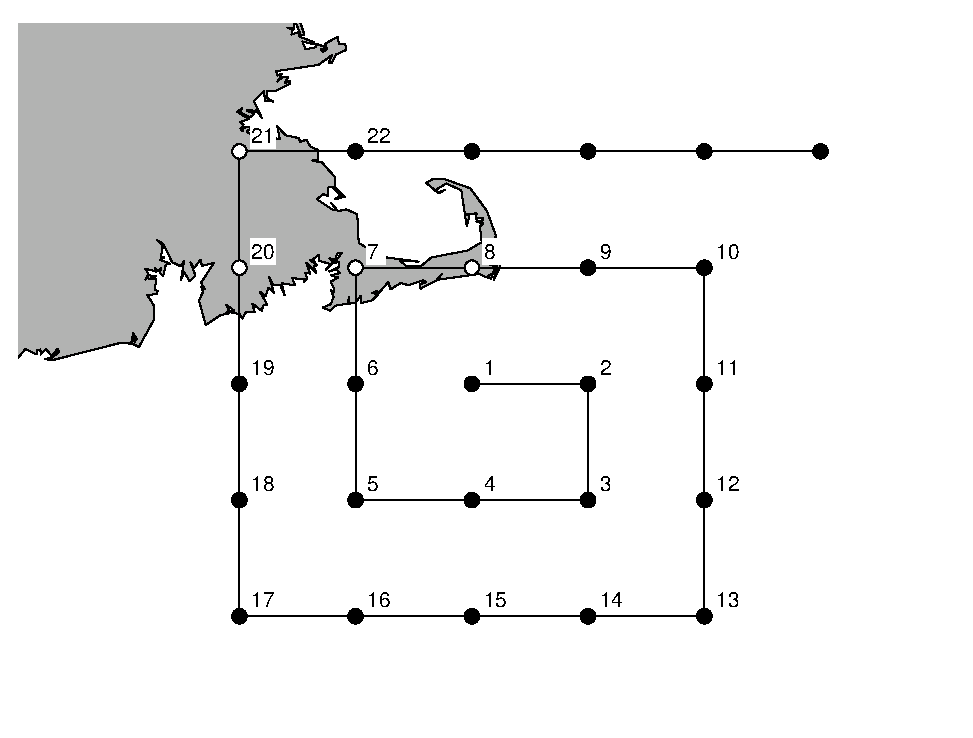
\epsfig{file=./num/wavetrack.eps,width=3.5in}
\caption{Example of a tracking spiral on a regular computational grid 
over a coastal domain featuring landmass (shaded). Black dots indicate 
active grid points and white dots indicate inactive (dry) grid points.}
         \label{fig:wavetrack} \botline
\end{center}
\end{figure}

\begin{equation}
    GoF_{i} = {\left( \frac{T_\mathrm{p} - \tilde{T}^\mathrm{n}_{\mathrm{p},i}}{\Delta T_\mathrm{n}} \right)}^2 + 
                     {\left( \frac{\theta_\mathrm{p} - \tilde{\theta}^\mathrm{n}_{\mathrm{p},i}}{\Delta\theta_\mathrm{n}} \right)}^2 +
                     {\left( \frac{H_\mathrm{m0} - \tilde{H}^\mathrm{n}_{\mathrm{m0},i}}{\Delta H_\mathrm{n}} \right)}^2\ \ ,
\label{eq:grdgof}
\end{equation} 

\noindent
where $\Delta T_\mathrm{n}$, $\Delta\theta_\mathrm{n}$ and $\Delta
H_\mathrm{n}$ are combining criteria \citep{art:WHD13}. If either of the first
two terms on the right hand side of (\ref{eq:grdgof}) exceed unity for the
closest match, the difference is considered too great and a new wave system is
assigned to that partition. Here, the search range for neighboring points is
set at 1, so that a maximum of four previously-associated neighbors can be
found (e.g. location 15 will have the previously processed neighbors 3, 4, 5
and 14). In some cases, iterative combining is required.

The next step is to correlate these wave systems over time. Each system $i$ at
the current time level $t$ is associated with its closest match amongst the
systems $j$ at the previous time level $(t-1)$. Three characteristics of the
wave systems are considered in this process, namely: (i) the spatial mean peak
wave period over the system, $\tilde{T}^\mathrm{s}_{\mathrm{p},t,i}$, with
$\mathrm{s}$ denoting the system mean, (ii) the spatial mean peak wave
direction, $\tilde{\theta}^\mathrm{s}_{\mathrm{p},t,i}$ and (iii) the number
of overlapping grid points between the two systems in geographical space
$\cap_{i,j}$. These characteristics are combined to form the following
GoF function:

\begin{equation}
    GoF_{i,j} = {\left( \frac{\tilde{T}^\mathrm{s}_{\mathrm{p},t,i} - \tilde{T}^\mathrm{s}_{\mathrm{p},t-1,j}}{\Delta T_\mathrm{s}} \right)}^2 + 
                       {\left( \frac{\tilde{\theta}^\mathrm{s}_{\mathrm{p},t,i} - \tilde{\theta}^\mathrm{s}_{\mathrm{p},t-1,j}}{\Delta\theta_\mathrm{s}} \right)}^2 +
                       {\left( \frac{N_{t-1,j} - \cap_{i,j}}{0.5N_{t-1,j}} \right)}^2\ \ ,
\label{eq:timegof}
\end{equation} 

\noindent
where $\Delta T_\mathrm{s}$ and $\Delta\theta_\mathrm{s}$ are combining
criteria, and $N$ is the total number of grid points in a system, see
\cite{art:WHD13}. In order to focus the tracking process on high-energy
regions in the wave field, the spatial mean period and peak direction values
of each system are weighted with the square of the significant wave
height. System $i$ at the current time level $t$ is assigned the system $j$
from the previous time level $(t-1)$ that minimizes (\ref{eq:timegof}). If any
of the three terms on the right hand side of (\ref{eq:timegof}) exceed unity
for the system that minimizes (\ref{eq:timegof}), a new system number is
assigned. For the last term, this implies a minimum spatial overlap
requirement, arbitrarily set at 50\%. This term mostly has an impact over
basin scale domains, where systems are typically smaller than the
computational area. In order to improve robustness, the details of identified
systems are stored for five time levels, after which the system association is
released.




\vssub
\subsection{~Nesting} \label{sub:num_nest}
\conthead{\ws}{H. L. Tolman}

\noindent
Traditionally, wave models only consider one-way nesting, with boundary data
from low resolution grids being provided to high resolution grids. This
approach has always been available in \ws, and is discussed in
\para\ref{sub:one_way}. In model version 3.14, a multi-grid wave model
driver was introduced, considering full two-way nesting between grids. This
approach is discussed in \para\ref{sub:two_way}. The illustrations below
consider regular grids, but the principles discussed are applicable to
curvilinear and triangular grids too.


% -------------------------------------------------------------
\vssub
\subsubsection{~Traditional one-way nesting} \label{sub:one_way}
\vssub

\begin{figure}
\begin{center}

\setlength{\unitlength}{0.001in}

\begin{picture}(3000,1800)(0,-1550)

\put(0200,-1200){\vector(1,0){2100}}
\put(2400,-1250){\makebox(400,100){\small space}}
\put(0300,-1300){\vector(0,1){1300}}
\put(0100, 0100){\makebox(400,100)[c]{\small time}}

\multiput(0300,-1200)(0,300){4}{\circle {50}}
\multiput(0600,-1200)(0,300){4}{\circle {50}}
\multiput(0900,-1200)(0,300){4}{\circle {50}}
\multiput(1200,-1200)(0,300){4}{\circle*{50}}
\multiput(1500,-1200)(0,300){4}{\circle {50}}
\multiput(1800,-1200)(0,300){4}{\circle {50}}
\multiput(2100,-1200)(0,300){4}{\circle {50}}

\put(0300,-0150){\makebox(600,100)[c]{`land'}}
\put(0900,-0200){\vector(-1,0){575}}

\put(1500,-0150){\makebox(600,100)[c]{sea}}
\put(1500,-0200){\vector(1,0){875}}
				       
\put(0900, 0050){\makebox(600,100)[c]{bound. data}}
\put(1100,-1200){\dashbox{50}(0200,1150){}}

\put(1050,-1550){\makebox(600,100)[c]{bound. scheme}}
\put(1200,-1400){\dashbox{25}(0300,1100){}}

\put(1550,-0750){\makebox(600,100)[l]{internal scheme}}
\put(1500,-0800){\vector(1,0){875}}

\end{picture}
\end{center}

\caption{Traditional one-way nesting approach as used in {\file ww3\_shel}.
         One-dimensional representation in space and time, symbols represent
         grid points.} \label{fig:nest1}
\botline
\end{figure}


The conventional wave model program {\file ww3\_shel} considers a single wave
model grid. This program includes options to transfer boundary conditions from
large-scale runs to small-scale runs. Each run can simultaneous accept one
data set with boundary conditions, and generate up to 9 data sets with
boundary conditions. To assure conservation of wave energy with incompatible
depths and currents, the boundary data consists of energy spectra
$F(\sigma,\theta)$. The data file consists of spectra at grid points of the
generating run, and information needed to interpolate spectra at the requested
boundary points. The size of the transfer files is thus minimized if the input
points for a small-scale run are located on grid lines in the large-scale
run. When used as input, the spectra are interpolated in space and time for
every global time step $\Delta t_g$, using a linear interpolation of spectral
components. 

The numerical approach for including boundary data in a wave model is
illustrated in Fig.~\ref{fig:nest1}. Active boundary points are assigned in
the grid to separate sea points from land points or from otherwise deactivated
grid points. Between the active boundary points and sea points, a local
boundary scheme is applied (typically first order). In the internal sea points
of the model, the selected propagation scheme is used.

Practical aspect of the conventional one-way nesting approach are
discussed in more detail in Appendix~\ref{app:nest}.


% -------------------------------------------------------------
\vssub
\subsubsection{~Two-way nesting} \label{sub:two_way}
\vssub

Model version 3.14 includes an option to use the multi-grid or mosaic approach
to wave modeling with the the program {\file ww3\_multi} \citep{tol:Vict06a,
  tol:MMAB07b, tol:OMOD08b}. In this program, an arbitrary number of grids
with arbitrary resolutions is considered, with data exchange between grids at
each relevant model time step. The grids are given a rank number, where lower
rank corresponds to lower resolution, and equal rank corresponds to similar
resolution (but not necessarily equal resolution).  Three types of data
transfer between grids are considered. These are

\begin{itemize}
\item Transfer of data from lower to higher rank grids.
\item Transfer of data from higher to lower rank grids.
\item Transfer of data between grids with equal rank.
\end{itemize}

Data transfer from lower to higher ranked grids is accomplished by providing
boundary data to the higher ranked grid, as in the traditional one-way nesting
approach described in the previous section and in Fig.~\ref{fig:nest1}.

\begin{figure}
\begin{center}

\setlength{\unitlength}{0.001in}

\begin{picture}(3000,1900)(0,-1600)

\multiput(0300,-1400)(0,300){6}{\circle {50}}
\multiput(0600,-1400)(0,300){6}{\circle {50}}
\multiput(0900,-1400)(0,300){6}{\circle {50}}
\multiput(1200,-1400)(0,300){6}{\circle {50}}
\multiput(1500,-1400)(0,300){6}{\circle {50}}
\multiput(1800,-1400)(0,300){6}{\circle {50}}
\multiput(2100,-1400)(0,300){6}{\circle {50}}
\multiput(2400,-1400)(0,300){6}{\circle {50}}
\multiput(2700,-1400)(0,300){6}{\circle {50}}

\multiput(0450,-1550)(300,0){8}{\dashbox{50}(0000,1800){}}
\multiput(0150,-1250)(0,300){5}{\dashbox{50}(2700,0000){}}

\multiput(0400,-1450)(0,800){3}{\circle*{100}}
\multiput(1400,-1450)(0,800){3}{\circle*{100}}
\multiput(2400,-1450)(0,800){3}{\circle*{100}}

\put(895,-1055){\framebox(1010,810){}}
\put(900,-1050){\framebox(1000,800){}}
\put(905,-1045){\framebox(990,790){}}

\end{picture}
\end{center}

\caption{Concept for reconciling lower ranked grid with higher ranked grid in
         two-way nesting approach. $\circ$ and hashed lines represent the
         higher ranked grid points and grid boxes, respectively, $\bullet$ and
         solid lines represent lower ranked grid and central grid box.}
\label{fig:nest2}
\botline
\end{figure}


When this approach is combined with data transfer from higher to lower rank, a
full two way nesting approach is established. In {\file ww3\_multi} the data
at the lower ranked grids is reconciled with the data at the higher ranked
grids after the higher ranked grids have `caught up' in time with the lower
ranked grids.  Considering that the resolution of the lower ranked grid by
definition is lower that the resolution of the higher ranked grid, a natural
way to estimate the wave energy in the lower ranked grid $E_{l,i}$ from energy
in the higher ranked grid $E_{h,j}$ is

\begin{equation}
E_{l,i} = \sum w_{i,j} W_{h,j} \:\:\: , \label{eq:nest_hg1}
\end{equation}

\noindent
where $i$ and $j$ are grid counters in the two grids, and where $w_{i,j}$ are
averaging weights. The weights can be defined consistent with conservation of
wave energy as the surface of the grid box $j$ in the higher ranked grid that
covers the grid box $i$ in the lower ranked grid, normalized with the surface
of the lower ranked grid box $i$. This is illustrated in Fig.~\ref{fig:nest2}.
To avoid circular reconciliation, grid points in the lower ranked grid that
contribute to the boundary data in the higher ranked grid are not updated in
this manner.

\begin{figure}
\begin{center}

\setlength{\unitlength}{0.001in}

\begin{picture}(3000,1900)(0,-1600)

\multiput(0300,-1400)(0,300){5}{\circle {50}}
\multiput(0600,-1400)(0,300){5}{\circle {50}}
\multiput(0900,-1400)(0,300){5}{\circle {50}}
\multiput(1200,-1400)(0,300){5}{\circle {50}}
\multiput(1500,-1400)(0,300){5}{\circle {50}}
\multiput(1800,-1400)(0,300){5}{\circle {50}}
\multiput(2100,-1400)(0,300){5}{\circle {50}}

\multiput(0950,-1275)(0,300){5}{\circle*{50}}
\multiput(1250,-1275)(0,300){5}{\circle*{50}}
\multiput(1550,-1275)(0,300){5}{\circle*{50}}
\multiput(1850,-1275)(0,300){5}{\circle*{50}}
\multiput(2150,-1275)(0,300){5}{\circle*{50}}
\multiput(2450,-1275)(0,300){5}{\circle*{50}}
\multiput(2750,-1275)(0,300){5}{\circle*{50}}

\put(1325,-1500){\dashbox{25}(0400,1600){}}
\put(1300,  100){\vector(-1,0){1100}}
\put(1725,  100){\vector(1,0){1100}}
\put( 725,  150){\makebox(400,100)[c]{A}}
\put(1325,  150){\makebox(400,100)[c]{B}}
\put(1925,  150){\makebox(400,100)[c]{C}}

\end{picture}
\end{center}

\caption{Concept for reconciling grids with identical rank and therefore
         similar resolution. $\circ$ represents points of grid 1, $\bullet$
         represents grid 2.}
\label{fig:nest3}
\botline
\end{figure}


Overlapping grids with similar rank cannot use the above two-way nesting
technique to consistently exchanger data. Instead, all such grids are
propagated one time step, after which the grids are reconciled as is
illustrated in Fig.~\ref{fig:nest3} For grid 1 ($\circ$ in
Fig.~\ref{fig:nest3}) two areas can be distinguished. In area C, the influence
of the boundary has propagated into the grid since the last
reconciliation. The actual depth of penetration depends on the stencil width
of the numerical scheme, and the number of propagation time steps.  In areas A
and B, information from the boundary has not yet penetrated, and this area can
be considered as the `interior' of grid 1.  Similarly, area A represents the
boundary penetration depth for grid 2 ($\bullet$ in Fig.~\ref{fig:nest3})
whereas B and C represent the interior of grid 2.  A simple and consistent
reconciliation between grid 1 and 2 uses data from grid 1 exclusively in area
A (interpolating data from grid 1 to grid points in grid 2 as necessary), and
uses data from grid 2 exclusively in area C. In area B, where interior parts
of both grids overlap, a consistent solution can be found by using weighted
averages from both grids. Note that this approach is easily extended to
multiple overlapping grids.

Note that for explicit numerical propagation schemes and overlapping grids with
identical resolution and coinciding grid points, solutions for overlapping
grids and the compatible single grid can be identical, as long as the overlap
areas are sufficiently wide.

\vspace{\baselineskip} 
\noindent 
The two-way nesting techniques in {\file ww3\_multi} are largely automated.
Each grid is prepared individually, with its own preferred time stepping
information. Locations where each grid expects to get boundary data are marked
as in the one-way nesting approach. All other bookkeeping needed to implement
the two-way nesting techniques are automated, although some iterations may be
needed to assure that all input boundary points defined in each grid can be
provided with boundary data from other grids in the multi-grid application.
Alternatively, each grid can obtain data from an external data file as in the
traditional nesting approach. In the present implementation, each grid has to
obtain all boundary data from a single file, of from other grids in the
multi-grid application, but cannot receive data from file and grids
simultaneously. Details on the management algorithm developed to run all grid
simultaneously can be found in \citet[section 3.4]{tol:MMAB07b} or
\cite{tol:OMOD08b}, and will not be reproduced here.

Note that the grids used in {\file ww3\_multi} do not need to have the same
spectral discretization. Spectra are converted on the fly in {\file
ww3\_multi}. Details on the numerical techniques used for this approach can be
found in \citet[section 3.5.5]{tol:MMAB07b}.
Grid generation for multiple grids in such an approach can be cumbersome, and
consistency between grids is required for consistent model results. For this
reason automated grid generation utilities have been developed by
\cite{tol:MMAB07a, tol:OMOD08a}.

% \bpage
